\documentclass{report}
\usepackage{amssymb}
\usepackage[dvips]{graphicx}
\usepackage{verbatim}
\usepackage{html}


\usepackage{amsmath}
\usepackage{latexsym,amssymb}
\usepackage[mathscr]{eucal}
\usepackage{amsthm,amsxtra,amscd,upref}
\usepackage{layout,bm,dcolumn}
\usepackage{graphicx,color}
\usepackage{calc}

\usepackage{framed}

\newcommand{\DST}[1]{{\ensuremath{\displaystyle{#1}}}}
\newcommand{\DSF}[2]{{\ensuremath{\displaystyle{\frac{\DST{#1}}{\DST{#2}}}}}}

\newcommand{\vk}[1]{{\ensuremath{\underline{\bm{#1}}}}}
\newcommand{\mx}[1]{{\ensuremath{\bm{\mathsf{#1}}}}}
\newcommand{\lrb}[1]{{\ensuremath{\left({#1}\right)}}}
\newcommand{\lrs}[1]{{\ensuremath{\left[{#1}\right]}}}
\newcommand{\lrc}[1]{{\ensuremath{\left\{{#1}\right\}}}}
\newcommand{\lrv}[1]{{\ensuremath{\left|{#1}\right|}}}

\newcommand{\hell}{{\ensuremath{\hat{\jmath}}}}
\newcommand{\zell}{{\ensuremath{\mathfrak{z}}}}
\newcommand{\vM}[0]{{\ensuremath{\vk{M}}}}
\newcommand{\vr}[0]{{\ensuremath{\vk{r}}}}
\newcommand{\vq}[0]{{\ensuremath{\vk{q}}}}
\newcommand{\vh}[0]{{\ensuremath{\vk{h}}}}
\newcommand{\vkx}[0]{{\ensuremath{\vk{x}}}}
\newcommand{\vkxt}[0]{{\ensuremath{\vk{x}^t}}}
\newcommand{\vky}[0]{{\ensuremath{\vk{y}}}}
\newcommand{\vkyt}[0]{{\ensuremath{\vk{y}^t}}}

\newcommand{\vri}[1]{{\ensuremath{\vk{r}_{#1}}}}
\newcommand{\vrr}{{\ensuremath{\vk{r}}}}
\newcommand{\vqi}[1]{{\ensuremath{\vk{q}_{#1}}}}
\newcommand{\vqr}{{\ensuremath{\vk{q}}}}
\newcommand{\vhi}[1]{{\ensuremath{\vk{h}_{#1}}}}
\newcommand{\vhr}{{\ensuremath{\vk{h}}}}
\newcommand{\IMA}{{\ensuremath{\mathrm{i}}}}
\newcommand{\EE}{{\ensuremath{\mathrm{e}}}}
\newcommand{\half}{{\ensuremath{\frac{1}{2}}}}

%\newcommand{\deltay}{{\ensuremath{\delta_{y}}}}
\newcommand{\deltax}{{\ensuremath{\rho\cos(\beta)}}}
\newcommand{\deltay}{{\ensuremath{\rho\sin(\beta)}}}
\newcommand{\deltaz}{{\ensuremath{\delta_{z}}}}
\newcommand{\deltazs}{{\ensuremath{\widehat{\deltaz}}}}
\newcommand{\DD}[1]{{\ensuremath{\mathrm{d}{#1}\, }}}
\newcommand{\DDD}[2]{{\ensuremath{\mathrm{d}^{#1}{#2}\, }}}

\newcommand{\haf}{{\ensuremath{\scriptstyle{\frac{1}{2}}}}}
\newcommand{\unt}{{\ensuremath{\scriptstyle{\frac{1}{3}}}}}
\newcommand{\dut}{{\ensuremath{\scriptstyle{\frac{2}{3}}}}}
\newcommand{\xref}[1]{(\ref{#1})}
\newcommand{\eref}[1]{Eq.~(\ref{#1})}
\newcommand{\Beref}[1]{{\textcolor[rgb]{0,0,1}{Eq.~(\ref{#1})}}}
\newcommand{\eeref}[2]{Eqs.~(\ref{#1},\ref{#2})}
\newcommand{\eeeref}[3]{Eqs.~(\ref{#1},\ref{#2},\ref{#3})}
\newcommand{\aref}[1]{Appendix~\ref{#1}}
\newcommand{\sref}[1]{Sec.~\ref{#1}}
\newcommand{\cref}[1]{Chap.~\ref{#1}}
\newcommand{\tref}[1]{Tab.~\ref{#1}}
\newcommand{\fref}[1]{Fig.~\ref{#1}}
\newcommand{\Rref}[1]{Ref.~\cite{#1}}
\newcommand{\degC}{{\ensuremath{{}^{\mathrm{o}}}}}

\newcommand{\TT}{{\ensuremath{{2\theta}}}}
\newcommand{\TTz}{{\ensuremath{{{\TT}_{0}}}}}
\newcommand{\TTe}{{\ensuremath{{{\TT}_{e}}}}}
\newcommand{\TTB}{{\ensuremath{{{\TT}_{B}}}}}


























\begin{document}

\title{SLS Detectors\\ Frequently Asked Questions}
\author{Anna Bergamaschi}
\date{\today}
\maketitle
\tableofcontents
\clearpage
\chapter{SLS Detectors Software}


\section{Which programs can I use to control my detector?}

The complete software package is composed of several programs which can be installed (or locally compiled) depending on the needs:

\begin{itemize}
\item The \textbf{slsDetector shared and static libraries} which are necessary for all user interfaces. \\
  The class slsDetectorUsers can be used as API from your acquisition software (see separate documentation).
\item The \textbf{command line interfaces (sls\_detector\_put, sls\_detector\_get, sls\_detector\_acquire, sls\_detector\_help)}, which are provided to communicate with the detectors using the command line and eventually to the data receiver
\item The \textbf{data receiver (slsReceiver)}, which can be run on a different machine, receives the data from the detector and interfaces to the control software via TCP/IP for defining e.g. the file name, output path and return status and progress of the acquisition
\item The  \textbf{graphical user interface (slsDetectorGUI)} which provides a user friendly way of operating the detectors with online data preview
\item The  \textbf{calibration wizards (energyCalibrationWizard, angularCalibrationWizard)} to analyze the data and produce the energy or angular calibration files
\end{itemize}

\section{How can I control many detectors in parallel or independently?}

For most users the detector will be composed by a single module. Therefore all configurations of the detector will refere to that single entity.

However, for some experiments it is necessary to concatenate the data from several detector controllers, and sometimes (e.g. MYTHEN) each controller can control many modules. This should be transparent to the user since most parameters will be identical for all controllers (e.g. exposure time, energy threshold etc.), except for the configurations specific to the controller (e.g. hardware configuration).\\
In principle it is possible to combine controllers of different type (e.g. MYTHEN, GOTTHARD, EIGER) but the user should then evaluate if it really makes sense to control such different systems in parallel.

In other cases, several SLS detectors will independently acquire data during the same experiment. In this case it will be necessary to be able to seperately control them.

The detectors can be controlled in parallel from several PCs (clients). However it is important the the configurations match on all of the them such that no conflict arise. Eventually a detector can be locked to a specific control PC, still different users interfaces (command line, GUI) can be used in parallel.

A sketch of a possible complex detector configuration is shown in figure~\ref{fig:multidet}

%\section{Detector indexes}

For this reason and index is assigned to each detector. If a single detector is used, as in most cases, the index will be omitted and defaults to 0.\\
To control the other detectors the index cannot be omitted!\\


An index will also be assigned to each controller within a detector. However the user normally will not need to address single controllers, except for the most advanced settings which can be left to configuration files.\\


Finally each module within a controller has an internal index. However in general it is not required that the user is aware of the system architecture and, if needed (rarely), the modules can simply be addressed sequentially starting from controller 0.



\begin{figure}
\caption{Scketch of a possible complex system architecture composed of several detector, each consisting in many controllers eventually controlling several modules.}\label{fig:multidet}
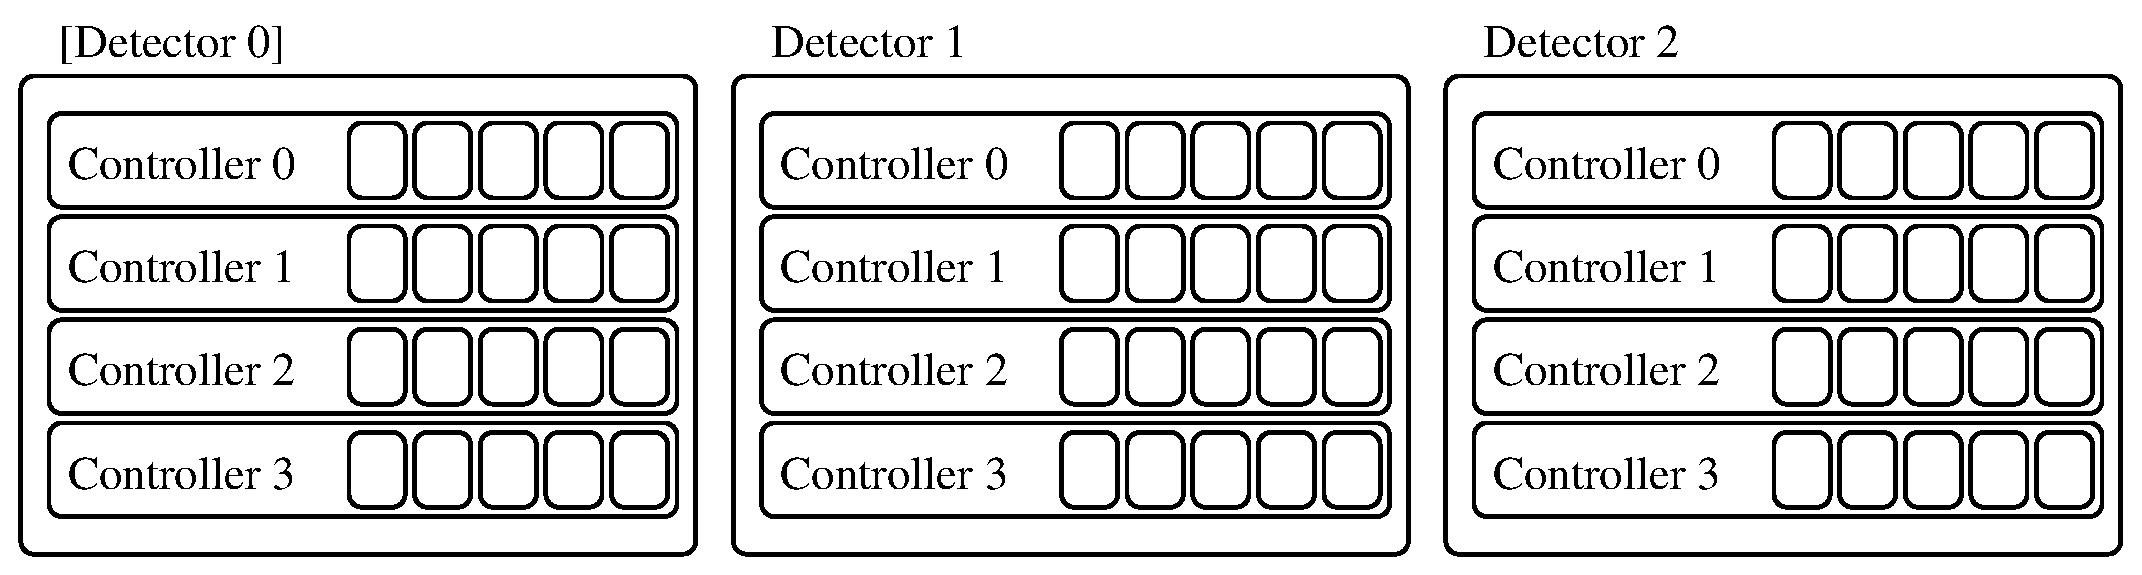
\includegraphics[width=\textwidth]{multi_detector}
\end{figure} 

\subsection{Examples}

For MYTHEN, if one needs to control 6 modules, the system can either be composed by and MCS6 with 6 modules (1 detector, 1 controller, 6 modules), or by 6 MCS1 (1 detector, 6 controller, 1 module each). After apppropriate configuration of the system, the interface to the user will be the same for both systems.

For GOTTHARD, one module corresponds to one controller. A detector will have the smae number of controllers and modules.

For EIGER, one module consists in two controllers. Fo a multi-module system, the number of controllers will increase accordingly, but should be left to a configuration file.

You will need to configure more than one detector, only in case you want to operate several detectors independently.


\section{How can I configure the data receiver?}

For slower acquisitions, the detector will return the data to the control PC over TCP/IP (e.g. MYTHEN).

However, for faster frame rates (e.g. GOTTHARD, EIGER) the controllers will return the data to a data receiver i.e. a process specifically designed to receive the data from the controller over a GBit network and save them to disk. \\
The data receiver can run on any machine (e.g. a file server) accessible by both the control PC and the detector controller, as sketched in figure~\ref{fig:datareceiver}. A data receiver process must be configured for each controller. Normally, to avoid performance loss it is better if different data receivers run on different machines.

\begin{figure}
\caption{Scketch of the communication between the control PC, the detector and the data receiver.}\label{fig:datareceiver}
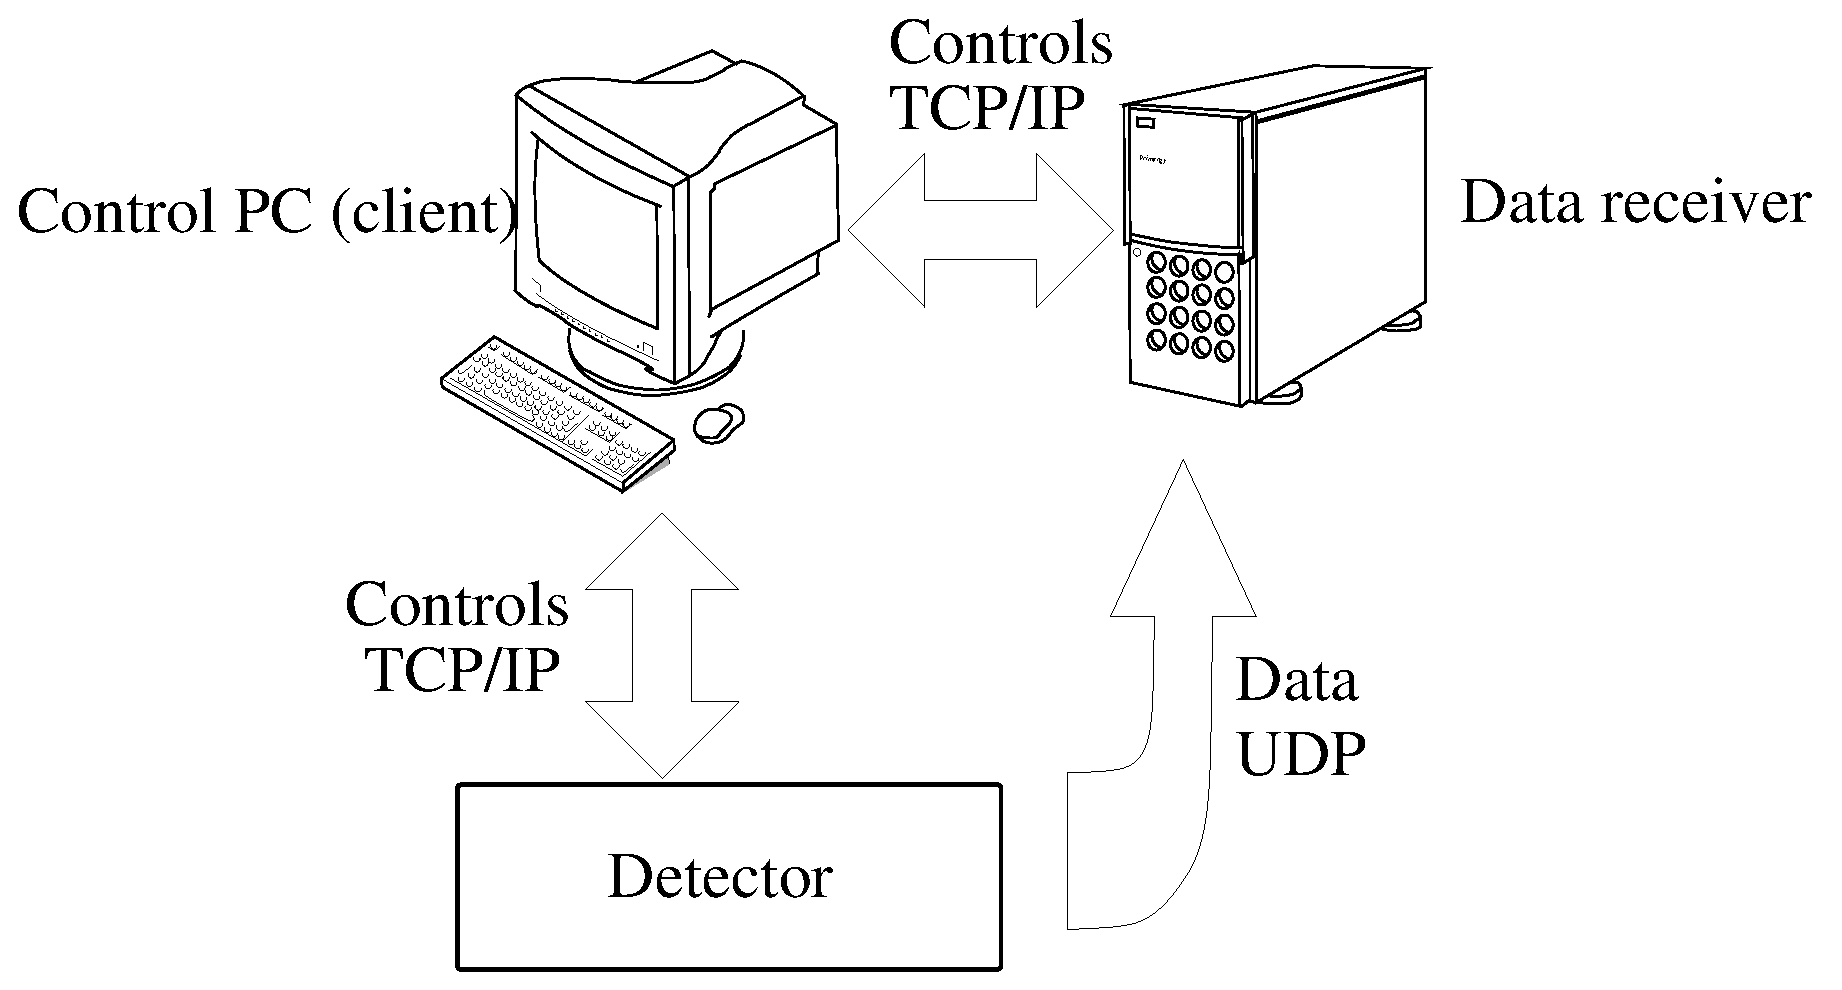
\includegraphics[width=\textwidth]{data_receiver}
\end{figure} 


 
To setup the system, you should configure:
\begin{description}
\item[Client-Detector TCP/IP connection] i.e. for each controller hostname  or IP address  (\textit{hostname}) and communication port (\textit{port}, use default).
\item[Client-Receiver TCP/IP connection] i.e. hostname or IP address of the data receiver (\textit{rx\_hostname}) and communication port (textit{rx\_tcpport}, use default).
\item[Detector-Receiver UDP connection] i.e.  for each controller IP address of the receiver network interface (\textit{rx\_udpip}) and communication port (\textit{rx\_udpport}) used for receiveing the data. By detfault the IP address of the TCP/IP receiver interface will be used also for the UDP conenction. Editing the UDP network interfaces and ports is useful if several controller are sending data to a single receiver (not reccomended to avoid performance loss).\\
A MAC  (\textit{detectormac}) and IP address (\textit{detectorudpip}) should also be assigned to the controller network interface used for the UDP communication, but the default values can normally be used unless firewalls are defined between the detectors and the receiver.
\end{description}
All these configurations are normally left to the configuration file and should not be changed dynamically by the user.

After starting the data receiver process and correctly configuring the client and the detector, this architecture should be completely transparent for the user, except that the output file path must be properly configured from the client for the data receiver machine (easiest is that the disk is mounted for both machines in the same location).\\
The client will take care of communicating with the data receiver and the detector. A feedback about the progress of the acquisition and a preview of the data being acquired can also be obtained by the client from the data receiver.



\section{What are settings and calibration files for?} \label{sec:trimdir}

The analog characteristics of the detector have to be initialized in order to define the noise and the dynamic range which need to be used for the measurements. These parameters have a different meaning for analog or digital detectors, but in both cases some predefined voltage levels and current (we call them \textit{settings}) must be laoded to the detector. Moreover, there are some parameters that are custom to single detectors or modules (e.g. the trimbits). All these settings are stored in some settings file, which are organized in a \textit{settingsdir} with a definite architecture, where the software will look for the files to load to the detector whaen changing its settings.

In addition to that, in a single photon counting detector the threshold is set as a voltage level for the comparator, but for the user it is useful to have a direct conversion to the energy level. For this, after a proper calibration of the detector (see specific documentation) calibration file are generated in order to convert threshold in volts to keV. Also in this case the directory \textit{caldir} where the calibration files are stored must be defined ad organized with a proper architecture, suche that the software can find the calibration coefficients for settings the threshold.\\
Normally \textit{settingsdir} and \textit{caldir} can be the same, but have been left separate for flexibility.

The \textit{settingsdir} and \textit{caldir} should be properly configured for your detector either in a configuration file (for use with text clients, GUI or API) or dynamically (works only for the text clients).

In the following, the architecture of the \textit{settingsdir} and \textit{caldir} is described for the different detectors.

\subsection{MYTHEN}
For mythen, an example of \textit{settingsdir} and \textit{caldir} is  given in the software package by the directory \verb=trimdir=. 
Since these directories are customized by producing trimbit files and calibration for each detector, make sure not to overwrite yours every time you upgrade the software.

\textit{settingsdir} should contain three subdirectories \verb=standard=,  \verb=fast= and  \verb=highgain= containing respectively the trimfiles \verb=standard.trim=,  \verb=fast.trim= and  \verb=highgain.trim= which contain the correct voltage settings for the detector although all the individual channel thresholds set to 0. The original files contained in the package should be used, infact in case of error the detector would not recognize the correct settings.\\
The default trimbit files for each file will be stored in the directory according to the settings with the name \verb=noise.snxxx= where \verb=xxx= is the module serial number.\\

\textit{caldir} should contain three subdirectories \verb=standard=,  \verb=fast= and  \verb=highgain= containing respectively the trimfiles \verb=standard.cal=,  \verb=fast.cal= and  \verb=highgain.cal= which contain an average calibration of the modules for the diffrent settings. However this can different from the correct one for each individual module even of several kev and therefore it is very important to perform an energy calibration on a module basis.\\
The default calibration files for each file will be stored in the directory according to the settings with the name \verb=calibration.snxxx= where \verb=xxx= is the module serial number.


\subsection{GOTTHARD}
A \textit{settingsdir} should be configured, as the directory  \verb=settings= in this software package.\\
It must contain the subdirectories \verb=dynamicgain=, \verb=gain1=,  \verb=gain2=,  \verb=gain3=,  \verb=highgain=,  \verb=lowgain=,  \verb=mediumgain=, and   \verb=veryhighgain= in order to properly configure the GOTTHARD detector using the various gain settings.


\section{How should a configuration file look like?}

A configuration file is a list of command necessary to properly configure your detector systems, with default valuee for some parameters and other settings that the users should normally not change dinamically.
For this reason most of the commands present in the configuration file cannot be modified when using the API.\\
The syntax of the configuration file is exactly the same as in the comman line interface, therefore you can refere to that documentation to edit the files.\\
The configuration files look different for the different detector types. Examples of configuration files can be found in the examples directory.

\section{What is the meaning of the file name?}
The final file name will be: \\
\textit{outdir/prefix}\verb=[_d=$d$\verb=][_S=\textit{v0}\verb=][_s=\textit{v1}\verb=][_p=\textit{p}\verb=][_f=\textit{f}\verb=]_=\textit{i}\verb=.=\textit{ext}\\
where: \\
\textit{outdir} is the output directory path;\\
\textit{prefix} is the chosen prefix for the file name;\\
\textit{d} is the detector index, in case of data receiver and more than one detector;\\
\textit{v0} is the scan0 variable with the desired precision, if scan0 is enabled;\\
\textit{v1} is the scan1 variable with the desired precision, if scan1 is enabled;\\
\textit{p} is the position index, if different positions are configured;\\
\textit{f} is the frame index of the first frame stored in the file, if many frames and cycles are configured;\\
\textit{i} is the file index;\\
\textit{ext} is the file extension e.g. \textit{.raw} for MYTHEN raw data, \textit{.dat} for MYTHEN processed data.

\section{Which is the sequence of the acquisition flow?}

The software gives the  possibility to setup several loops, actions and scan utilities which are then handled during the acquisition. 
The software will also take care to generate the file names  and increment the indexes accordingly.\\

Figure~\ref{eq:acqflow} shows in which sequence the various scripts and loops are executed when calling the acquire command. The loops are drawn using the $\Updownarrow$ symbol, while the scripts using the  $\Rightarrow$.


\begin{displaymath} \label{eq:acqflow}
%%%%%%%%%%%%%%%%%%%%%8
  \textrm{\textbf{MEASUREMENTS}} \\
 \left\Updownarrow \,
    \begin{array}{l} \\
  %   \textrm{Measurement loop} \\
  %   \\
%%%%%%%%%%%%%%%%%%%%%7
    % \left[ 
   %  \,
           \begin{array}{l} %\\
        	  \Rightarrow  \,  \textrm{Start script} \\
	   \\
%%%%%%%%%%%%%%%%%%%%%6
                    \textrm{\textbf{SCAN0}}
           \left\Updownarrow 
     \,
	          \begin{array}{l} \\
                 	  \Rightarrow \,  \textrm{Scan0 script} \\
           %        \textrm{Scan 0 level} \\
		   \\
%%%%%%%%%%%%%%%%%%%%%5
     
                    \textrm{\textbf{SCAN1}}      \left\Updownarrow  
     \,
	          \begin{array}{l} \\
                %   \textrm{Scan 1 level} \\
		 %  \\
%%%%%%%%%%%%%%%%%%%%%4
          % \left[  
   %  \,
	          \begin{array}{l} %\\
                 	  \Rightarrow \,  \textrm{Scan1 script} \\
                 	  \Rightarrow \,  \textrm{Script before} \\
		   \\
%%%%%%%%%%%%%%%%%%%%%3
     %      \left\Updownarrow       \,
	          \begin{array}{l} \\
                    \textrm{\textbf{POSITIONS}} \left\Updownarrow  \,	  
%%%%%%%%%%%%%%%%%%%%%2
	          \begin{array}{l} \\
             	  \Rightarrow \,     \textrm{Header before script} \\
		   \\
%%%%%%%%%%%%%%%%%%%%%1
       
                   \textrm{\textbf{CYCLES}}     \left\Updownarrow  \,
	          \begin{array}{l} \\
		  \\
%%%%%%%%%%%%%%%%%%%%%0
		  \textrm{\textbf{FRAMES}}    \left\Updownarrow  \right. \\ 
		  \\
%%%%%%%%%%%%%%%%%%%%%%%%%%0
		  \\
		  \end{array}
		  \right. \\ 
		  \\
%%%%%%%%%%%%%%%%%%%%%%%%%%1
        	  \Rightarrow \,  \textrm{Header after script}\\
		  \\
		  \end{array}
		  \right. \\ 
%%%%%%%%%%%%%%%%%%%%%%%%%%2
\\
\\
\\
           \end{array}
%	   \right. I see the digitest works fine, and this is good news.

		  \\ 
	 %  \\
%%%%%%%%%%%%%%%%%%%%%%%%%%3
	  \Rightarrow \, \textrm{Script after} \\
%\\
                   \end{array}
	  % \right. \\ 
	   \\
%%%%%%%%%%%%%%%%%%%%%%%%%%4
\\
                   \end{array}
	   \right. \\ 
\\
	   \\
%%%%%%%%%%%%%%%%%%%%%%%%5
\\
                   \end{array} 
	   \right. \\
	   \\
%%%%%%%%%%%%%%%%%%%%%%%%6
	  \Rightarrow	\,   \textrm{Stop script} \\
\\
            \end{array} 
 %     \right. \\
 %     \\
%%%%%%%%%%%%%%%%%%%%%%%%7
\\
      \end{array}  
\right. 
%%%%%%%%%%%%%%%%%%%%%%%%8
\end{displaymath}


If you prefere to handle the acquisition from your acquisition enviroment, simply leave al scripts and scans disabled and call the acquition from your acquisition enviroment. \\
Only the frames and cycles loops are defined in firmware and guarantee a precise timing of the acquisition which cannot replaced by any other method (you can synchronize to your beamline by hardware connection of the IO signals as described in~\ref{sec:timing}).

Hereafter a description of the meaning of the various loops:
\begin{description}
\item[Measurement loop] executes offline several times the entire sequence of the acquisition. At the end of each measurement the \textit{file index} is incremented.

\item[Scan 0 loop]
  is a high level scan loop which can be used e.g to loop on an enviroment variable (temperature, humidity...) or even to change sample.\\
 The list of steps or range of the \textit{scan0 variable} must be set as scan0steps or scan0range. For small steps of the scan variable, avoid overwriting of the files specifying all the necessary digits in the filename by properly setting the precision with scan0prec.

\item[Scan 1 loop]
  is a low level scan loop which can be used e.g to loop on an enviroment variable (temperature, humidity...) or to move the sample in case of radiation damage.\\
 The list of steps or range of the \textit{scan1 variable} must be set as scan1steps or scan1range. For small steps of the scan variable, avoid overwriting of the files specifying all the necessary digits in the filename by properly setting the precision with scan1prec.

\item[Position loop]
 The detector is moved in the angular positions specified by the positions command.\\
 The command for moving the detector should be defined as described in~\ref{sec:usersFunc}.\\
 All data acquired during a position loop will be merged together, unless the number of positions is set to 0. In this case single frames will be converted to angle without merging.\\
 Avoid using the position loop together with many frames/cycles.

\item[Cycles loop] is executed in real time and defines e.g. the number of triggers that will be accepted. The total number of images will be given by frames times cycles.

\item[Frames loop] is executed in real time and defines e.g. the images acquired per trigger. The total number of images will be given by frames times cycles.
\end{description}

Executing a script simply consists in a system call with the arguments specified below. The various scripts are executed only if they are enabled and different than \textit{none}. \\
The scripts must be executable and the capability of parsing the arguments passed by the acquition program is left to the user writing the scripts. some example scripts writte in awk can be found in the examples directory.\\
Hereafter a short description of how the scripts are called and with which options:
\begin{description}

\item[Start script]
     is executed at the very beginning of the measurement and can be used e.g. to initialize all the devices needed for the acquisition or open the beamline valves. The script is executed as:\\
      script  nrun=i par=p\\
      where i is the  \textit{file index} and p is the \textit{start script parameter}.

\item[Scan0 script]
  There are a few predefined scan modes i.e. \textit{threshold} changing the detector threshold in DAC units, \textit{energy} chaning the calibrated detector threshold in eV, \textit{trimbits} chaning the trimbits of the detector (advanced: do not use) and \textit{position} changing the detector position (if the motor movement is correctly setup as described in~\ref{sec:usersFunc}). Otherwise the scan0script is executed as:\\
 script nrun=i fn=fn var=v par=p\\
  where i is the  \textit{file index}, fn is the \textit{file name}, v is the value of the \textit{scan0 variable} at the present step of the scan0 loop and  p is the \textit{scan 0 script parameter}.

\item[Scan1 script]
  There are a few predefined scan modes i.e. \textit{threshold} changing the detector threshold in DAC units, \textit{energy} chaning the calibrated detector threshold in eV, \textit{trimbits} chaning the trimbits of the detector (advanced: do not use) and \textit{position} changing the detector position (if the motor movement is correctly setup as described in~\ref{sec:usersFunc}). Otherwise the scan1script is executed as:\\
 script nrun=i fn=fn var=v par=p\\
  where i is the  \textit{file index}, fn is the \textit{file name}, v is the value of the \textit{scan1 variable} at the present step of the scan1 loop and  p is the \textit{scan 1 script parameter}.

\item[Script before]
  is called just before the beginning of the data taking and can be used e.g. to open the shutter.
  The script is executed as:\\
  script nrun=i fn=fn par=p sv0=v0 sv1=v1 p0=p0 p1=p1 \\
  where i is the  \textit{file index}, fn is the \textit{file name}, p is the \textit{script before parameter}, v0 and v1 are the  values of the \textit{scan0 and scan1 variables} at the present step of the scan loops and  p0 and p1 are the \textit{scan0 and scan1 script parameters}.
  

\item[Header before script]
    is called before every step of the data taking (i.e. for each position, but at the beginning of the frames train if several acquisition have been programmed in real time) and can e.g. be used to dump the exact settings of the detector and beamline to reproduce or analyze the data offline.
    The script is executed as:\\
    script nrun=i fn=fn par=p\\
    where i is the  \textit{file index}, fn is the \textit{file name}, and p is the \textit{header before parameter}.

\item[Header after script]
    is called after every step of the data taking (i.e. for each position, but at the end of the frames train if several acquisition have been programmed in real time) and can e.g. be used to dump the exact settings of the detector and beamline to reproduce or analyze the data offline.
    The script is executed as:\\
    script nrun=i fn=fn par=p\\
    where i is the  \textit{file index}, fn is the \textit{file name}, and p is the \textit{header after parameter}.

\item[Script after] 
  is called just after the end of the data taking and can be used e.g. to close the shutter.
  The script is executed as:\\
  script nrun=i fn=fn par=p sv0=v0 sv1=v1 p0=p0 p1=p1 \\
  where i is the  \textit{file index}, fn is the \textit{file name}, p is the \textit{script after parameter}, v0 and v1 are the  values of the \textit{scan0 and scan1 variables} at the present step of the scan loops and  p0 and p1 are the \textit{scan0 and scan1 script parameters}.
  
\item[Stop script]
     is executed at the very end of the measurement and can be used e.g. to switch off all devices. The script is executed as:\\
      script  nrun=i par=p\\
      where i si the \textit{file index} and p is the \textit{stop script parameter}.

\end{description}






\section{How can I synchronize my detector with the experiment?}\label{sec:timing}

The timing of the detector is always defined by an active detection time followed by a dead time during which the detector is read out. This read out time as a fixed duration depending on the detector type and its configuration (e.g. dynamic range) which limits the maximum frame rate achievable.\\
In the following is a list of the main parameters involved in the acquisition timing:
\begin{description}
\item[Exposure time] is the time during which the detector is detecting X-rays for each image (ignored is the timing mode is \textit{gating}).
\item[Period] is the period of the images acquired. If it is shorter than the exposure time plus readout time, it will be ignored.
\item[Delay after trigger] can be set as a delay between the trigger signal and the start of the detection time. 
\item[Number of gates] is used only in \textit{gating} mode and is the number of times that the gate is toggled before the detector is read out. Useful for stroboscopic measurements with gate period shorter than the minim acquisition period of the detector, otherwise can be left to 1.
\item[Number of frames] is the number of images to be acquired per cycle. Frames and cycles have the same meaning except in trigger mode, when frames means the number of images per trigger. The total number of images is frames time cycles.
\item[Number of cycles] is the number of times that the frames are acquired. Frames and cycles have the same meaning except in trigger mode, when cycles means the number of triggers that will be accepted. The total number of images is frames time cycles.
\item[Number of probes] is used in stoboscopic measurements when the period is longer than the minimum acquisition period, but shorter than the frame rate.\\
In this case the data can be summed in firmware. \\
Currently it is implemented for Mythen only. If probes is set to 0, works normallyreturning an image for each readout, otherwise set number of cycles to 1. The maximum number of probes that can be set is 3. The detector will return a number of image equal to the number of probes, where all frames are going to be accumulated. The total number of readouts is number of frames time probes and for  probes=1 the detector will return one image where all frames have been summed, for  probes=2 two images where every second frame has been summed (each image accumulates the number of frames), for probes=3 three images where every third image has been summed (each image accumulates the number of frames).\\
The returned images will always have 32~bit dynamic range, while the dynamic range if the detector defines the bit depth of the counters in rder to limit the readout time, if necessary.\\
The probes counter waorks also in trigger and gating modes.
\end{description}





\begin{figure}
\begin{center}
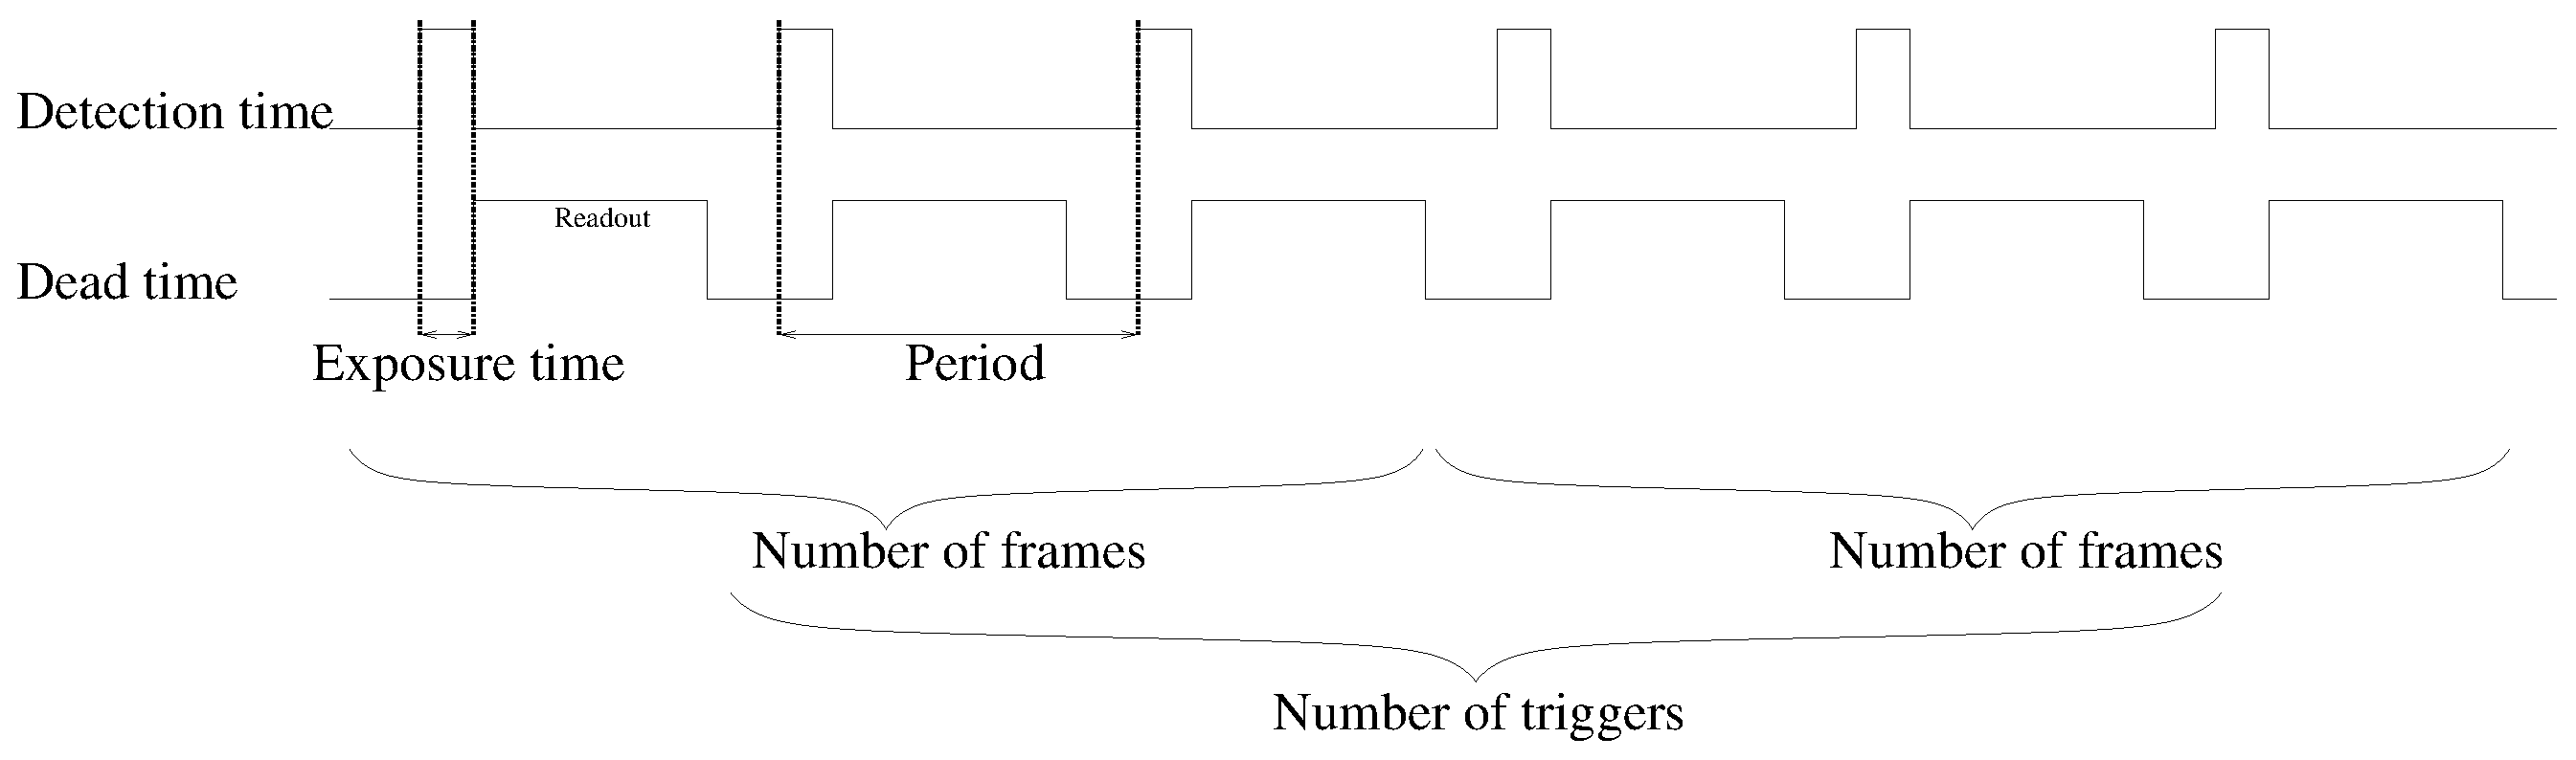
\includegraphics[width=\textwidth]{images/normal_acquisition.eps}
\end{center}
\caption{Auto timing: the detection time is defined by the exposure time and the period by period (if longer than exposure time plus readout time). The total number of images is frames (in the example 3) times cycles (in the example 2), and in this case there is no difference between the acquisition of the two.}\label{fig:autotiming}
\end{figure}

\begin{figure}
\begin{center}
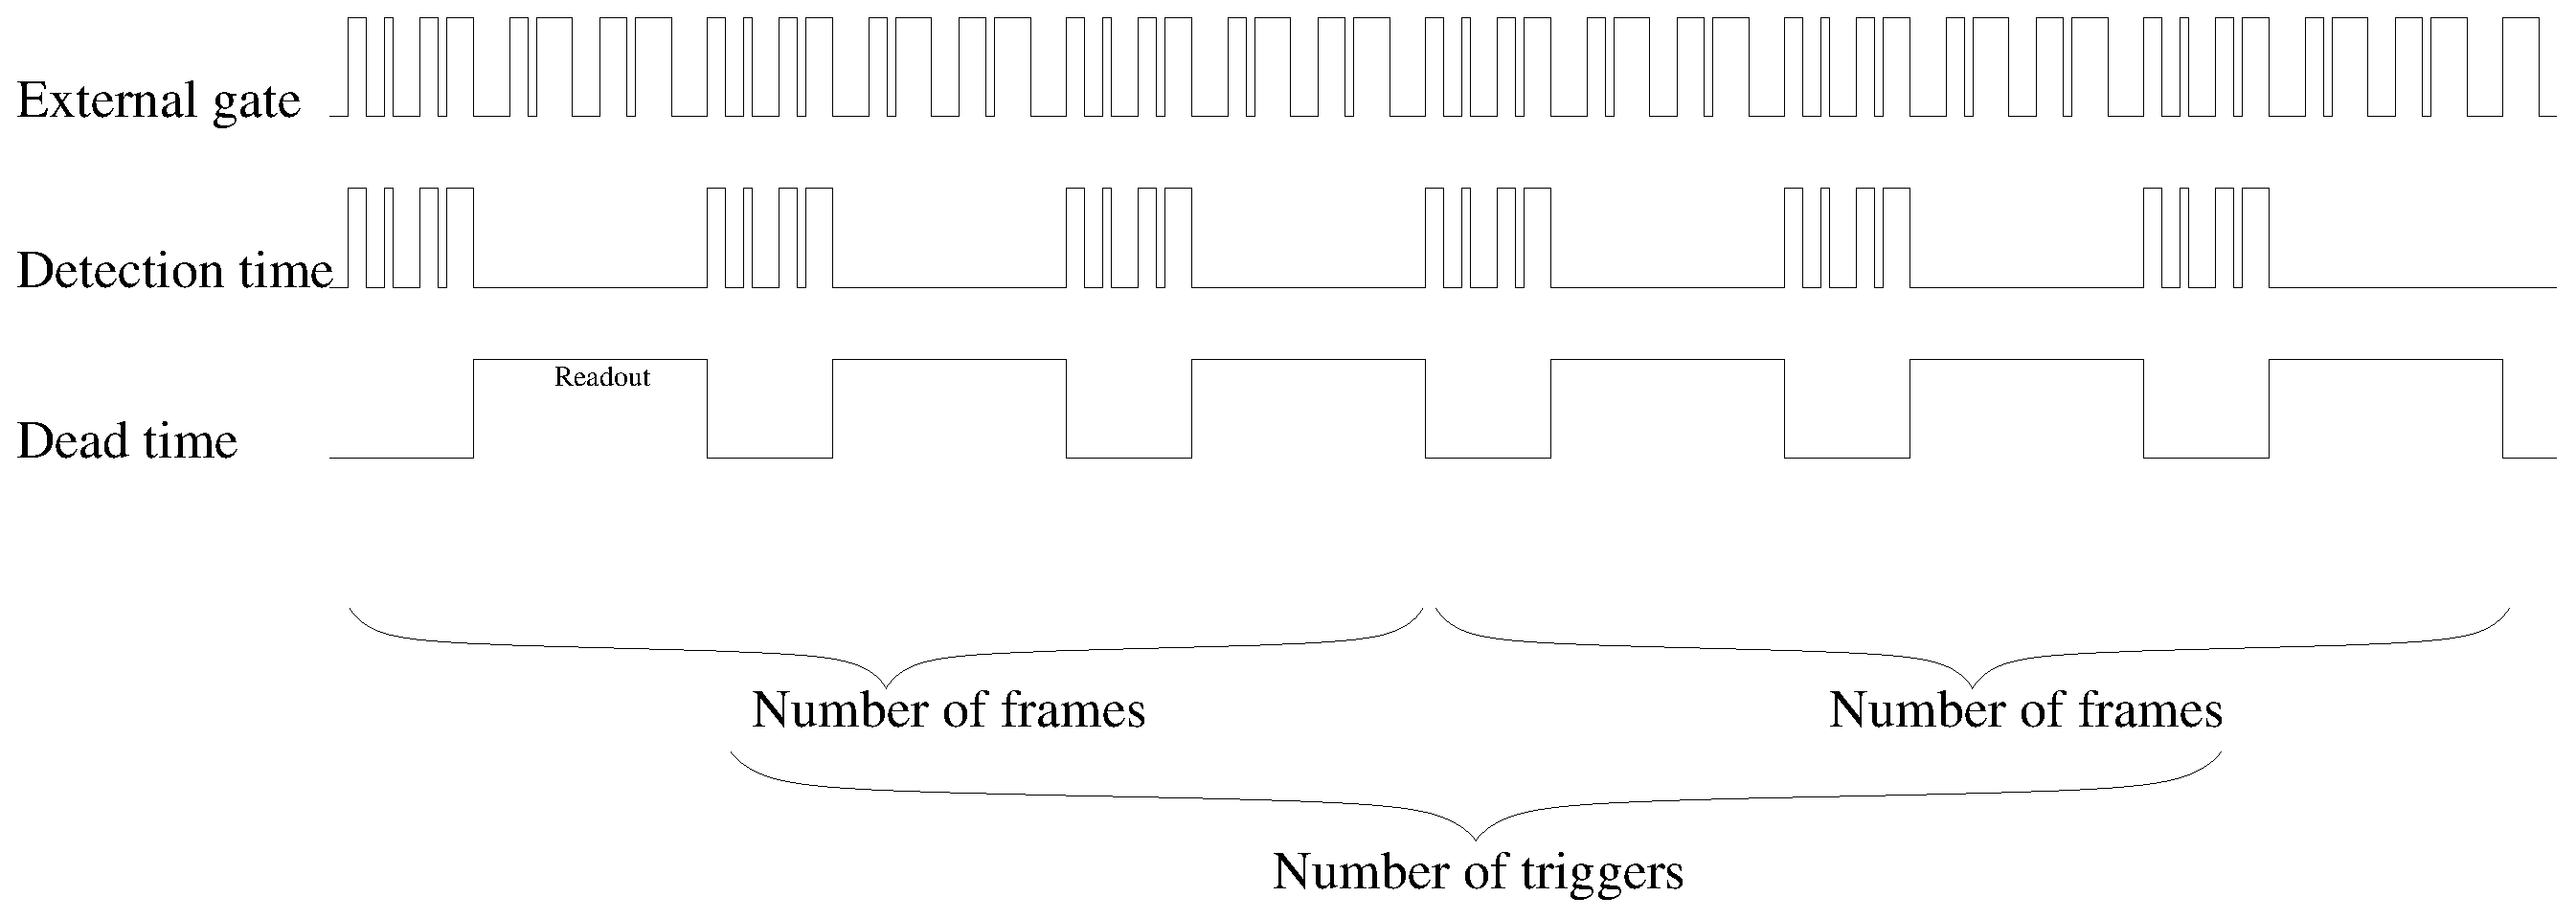
\includegraphics[width=\textwidth]{images/gated_acquisition.eps}
\end{center}
\caption{Gating mode: the detector acquires for a number of gates define by the  user (in this case 4) before being read out, independently on the timing of the gates. The detector remains insensitive during the readout time and then starts being active again. External gates given during the readout time are ignored. The total number of images is frames (in the example 3) times cycles (in the example 2), and in this case there is no difference between the acquisition of the two. The polarity of the external gate signal can be defined by the user through the \textit{external signal flag} (in the example active high).}\label{fig:gating}
\end{figure}



\begin{figure}
\begin{center}
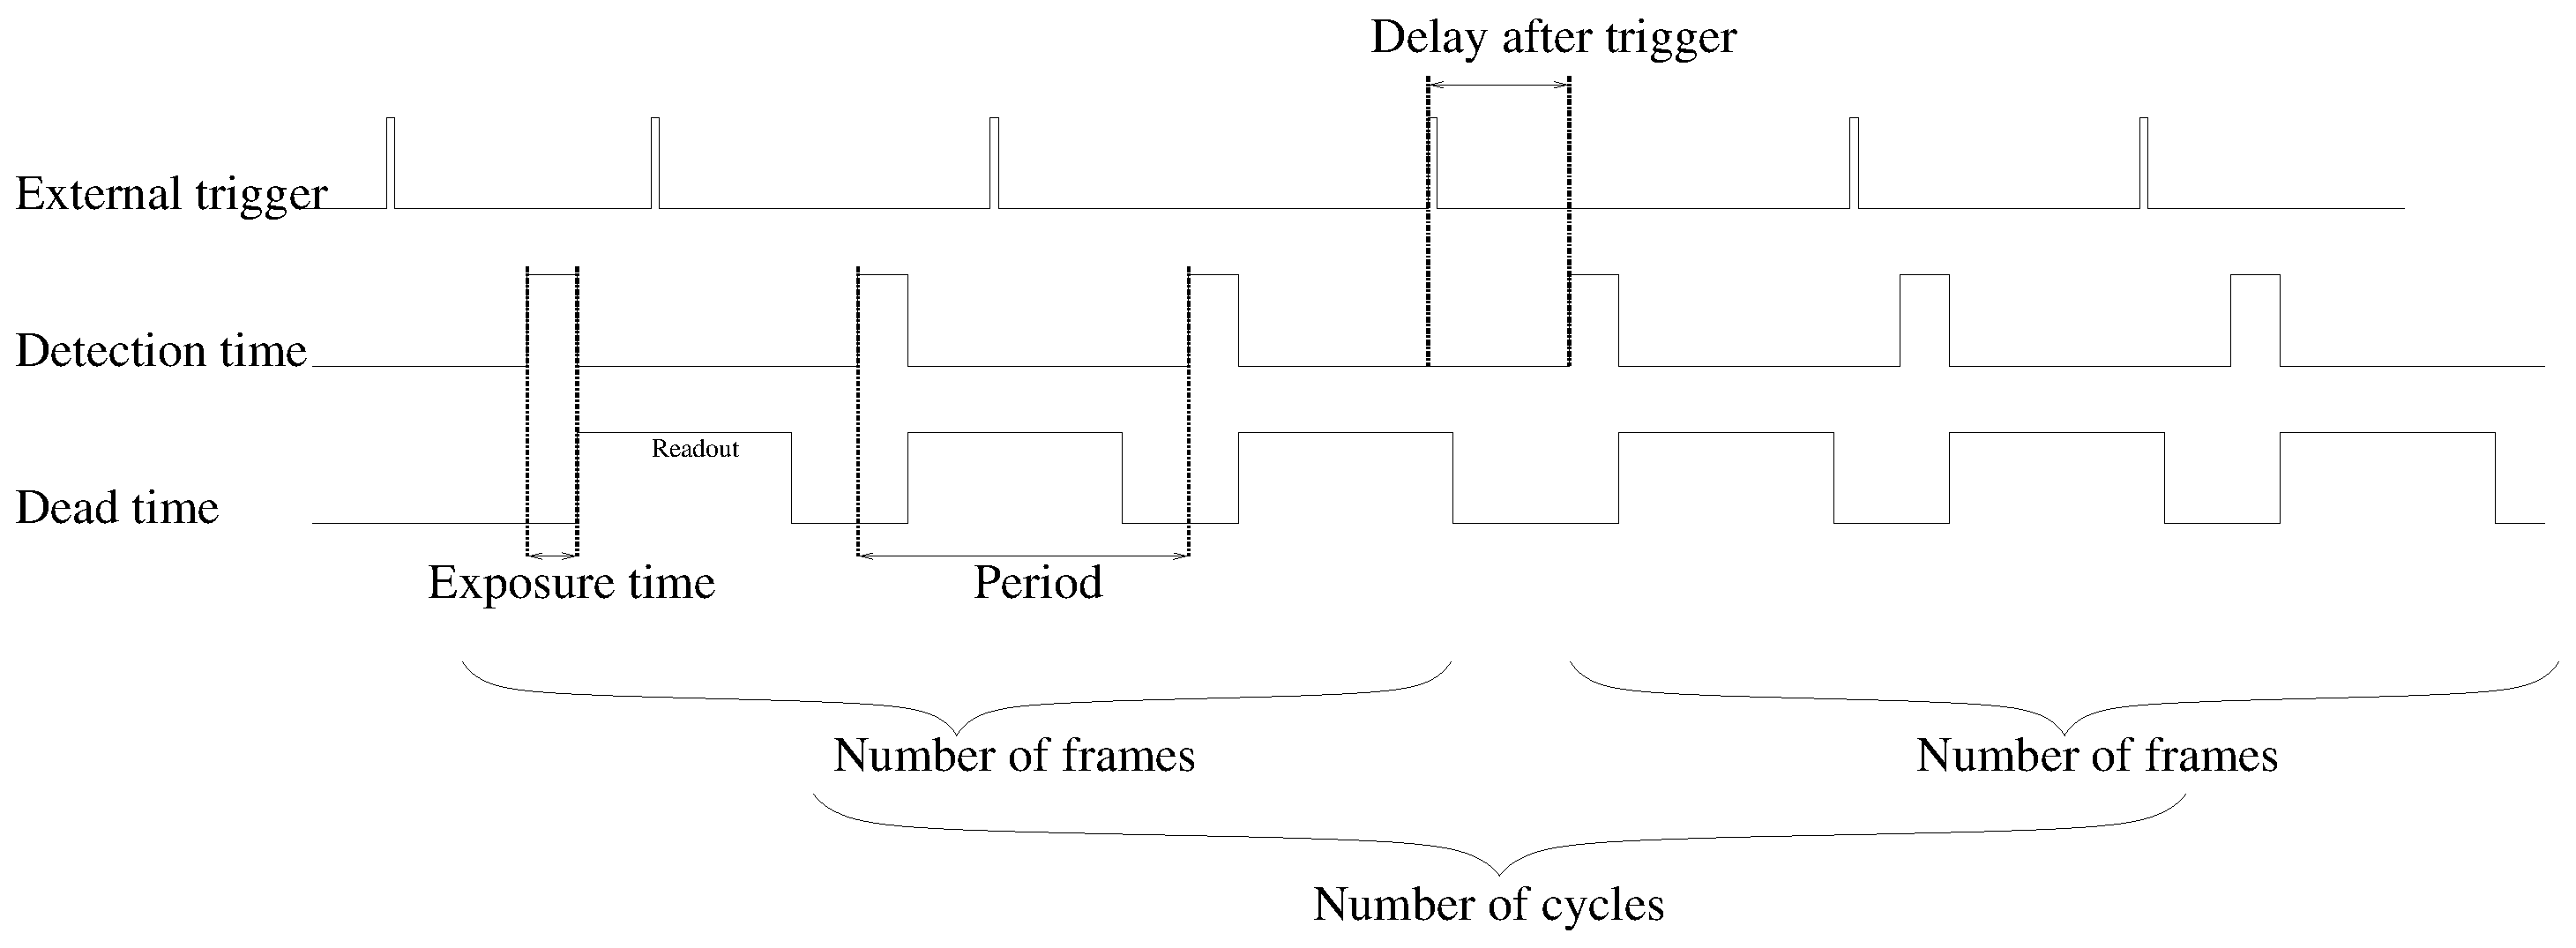
\includegraphics[width=\textwidth]{images/trigger_acquisition.eps}
\end{center}
\caption{Trigger mode: the external trigger signal defines the start of the beginning of the acquisition, which starts after the delay set by the user. For each trigger, the number of frames is acquired (in the example 3) and all trigger signals ignored. The number of trigger accepted is given by the number of cycles (in the example 2). The polarity of the external trigger signal can be defined by the user through the \textit{external signal flag} (in the example rising edge).}\label{fig:trig}
\end{figure}


\begin{figure}
\begin{center}
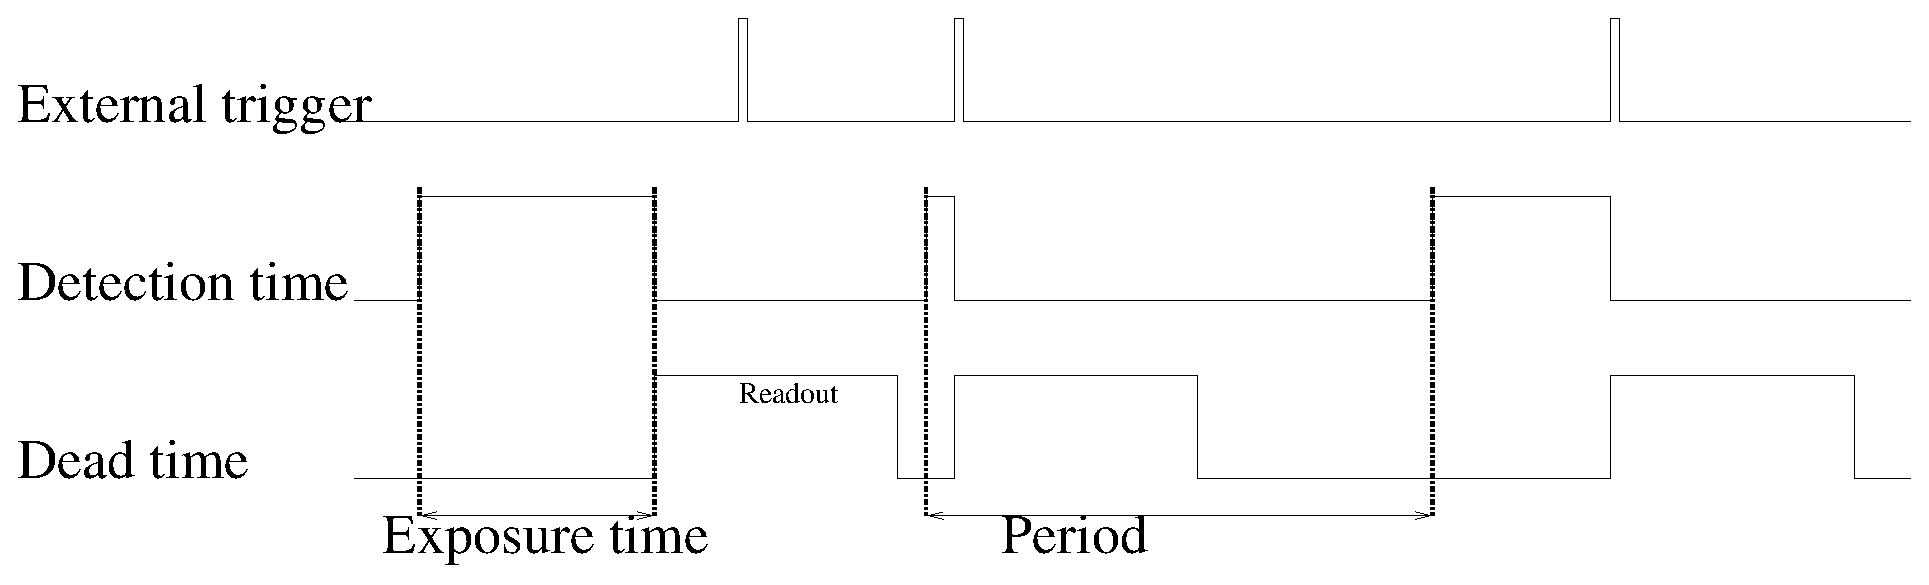
\includegraphics[width=\textwidth]{images/ro_trigger_acquisition.eps}
\end{center}
\caption{Read Out Trigger mode: the external trigger signal defines the beginning of the readout. The exposure time works as a time out for the waiting time for the trigger signal. The number of trigger accepted is given by the number of cycles (in the example 3) and it does not make sense to program more than one frame. The polarity of the external trigger signal can be defined by the user through the \textit{external signal flag} (in the example rising edge).}\label{fig:trig}
\end{figure}


\section{How can several controllers be synchronized?} \label{sec:sync}
If you are not performing time resolved measurements, you will probably not need any synchronization of the controllers: they will be started sequentially by the software and their acquisition will have a jitter of a few ms. \\
In the case you need a precise synchronization, on the other hand, hardware connection is required between the controllers through the external IO signals. The external signals used for this synchronization should be configured as \textit{sync} with the \textit{extsig} command. \\
In this case a \textit{master} controller should be defined for the acquisition which will the send the synchronization signal to the other controllers, while the other controllers will use them as inputs.\\
The type of synchronization can be\textit{gating} or \textit{trigger} depending if the synchronization signal will gate the slave detectors or trigegr the beginning of the acquisition. There are no particular reasons to chose one or the other method, except if the user finds out that one is more stable than the other.\\
Normally the configuration of the synchronization is configured inside the configuration file and should not be changed dynamically by the user.\\

After the configuration, the synchronization of the controllers will be completely transparent for the user, who will simply have to setup the timing parameters of the detector as a whole.

\section{How can the detector movement and position and I0 readout be customized for my beamline?} \label{sec:usersFunc}

The easiest way to allow the software to perform all the necessary normalization and angular conversion steps, is enable it to move your detector and read the encoder position and the value of the ionization chamber.\\
These functions are defines as callbacks and can be redifined by registering your own functions. This is normally a good method if you use the API or are willing to write your main client program.\\
Otherwise the simpleast way is to edit the file\\ 
\verb=slsDetectorSoftware/usersFunctions/usersFunctions.cpp= \\
where the default functions performing these actions are implemented and modify them to interface with your beamline hardware. The functions are written in C and are very simple to implement for anyone with some programming knowledge.\\
A simple high-level solution in case you need to maintain the software for several beamlines and don't want to recompile for all of them is to call external scripts.


\section{In which data format are written the data?} \label{sec:dataFormat}

For MYTHEN the data are writen in ASCII fomat, one file per frame, in columns, either channel number - counts for the \textit{.raw} files or angle (or channel number)-counts-error for the \textit{.dat} files.

For the other detectors the files are written in binary format, and must be decoded depending on the detector.

\subsection{GOTTHARD}
Each files contains 100 frames.
\begin{description}
\item[Normal mode]
Each frame is split into 2 packets of 1286 bytes each, where actual data is 1280 bytes each. Both the packets (incl header and footer) are written one after the other into the file.

Representation of each packet:
\begin{itemize}
\item
The first 4 bytes represents a number from which, the frame number and packet number can be derived.
If the number was 108601, increment it by 1 to get 108602.\\
Then this $(108602\&0xFFFFFFFE)>>1 = 54301$ is the frame number
and  $(108602\&0x1) =0$ is the packet number.\\
0 is the packet on the left and 1 is the packet on the right.\\
On a side note, when you use the data call back, we also give you the derived frame number as an argument.

\item Data of 1280 bytes. 16 bits per pixel.

\item  2 bytes of insignificant footer.
\end{itemize}

\item[Short Frame Mode]
One Frame has only one packet of 518 bytes, where actual data is 512 bytes.
\begin{itemize}
\item   first 4 bytes is the frame number. There is no increment like the previous ones.
\item   Data of 512 bytes.
\item   2 bytes of insignificant footer.
\end{itemize}

\end{description}

\subsection{EIGER}

\subsection{JUNGFRAU}


%\begin{comment}
\chapter{General questions about detectors}

\section{In which X-ray energy range can I use the detector?}

General remarks about sensor efficiency and electronic noise

\section{What is the electronic noise?}\label{sec:noise}


\section{What limits the maximum frame rate?}


%	\end{comment}

\chapter{Single photon counting detectors}


\section{Which detector settings should I choose?}

The choice of the operation settings is very important in order to obtain good quality data. 


Normally the user can follow these rules:
\begin{enumerate}
\item If the X-ray energy is lower than 8~keV the \textit{High gain} setting should be used. Since it is a slow mode of operation it is necessary to take care that the maximum count rate is lower than 100~kcounts/s for all channels (use filters to reduce the beam intensisty).
\item For energies higher than 8~keV, the \textit{Standard} setting is normally fine if the count rate can be kept lower than 300~kcounts/s for all channels (use filters to reduce the beam intensisty). 

\item In case a larger count rate is required in order to keep the acquisition time shorter, the \textit{Fast} setting must be selected. However the maximum count rate should never exceed 1~Mcounts/s   for all channels.
\end{enumerate}

\subsection{MYTHEN}


\begin{figure}
\begin{center}
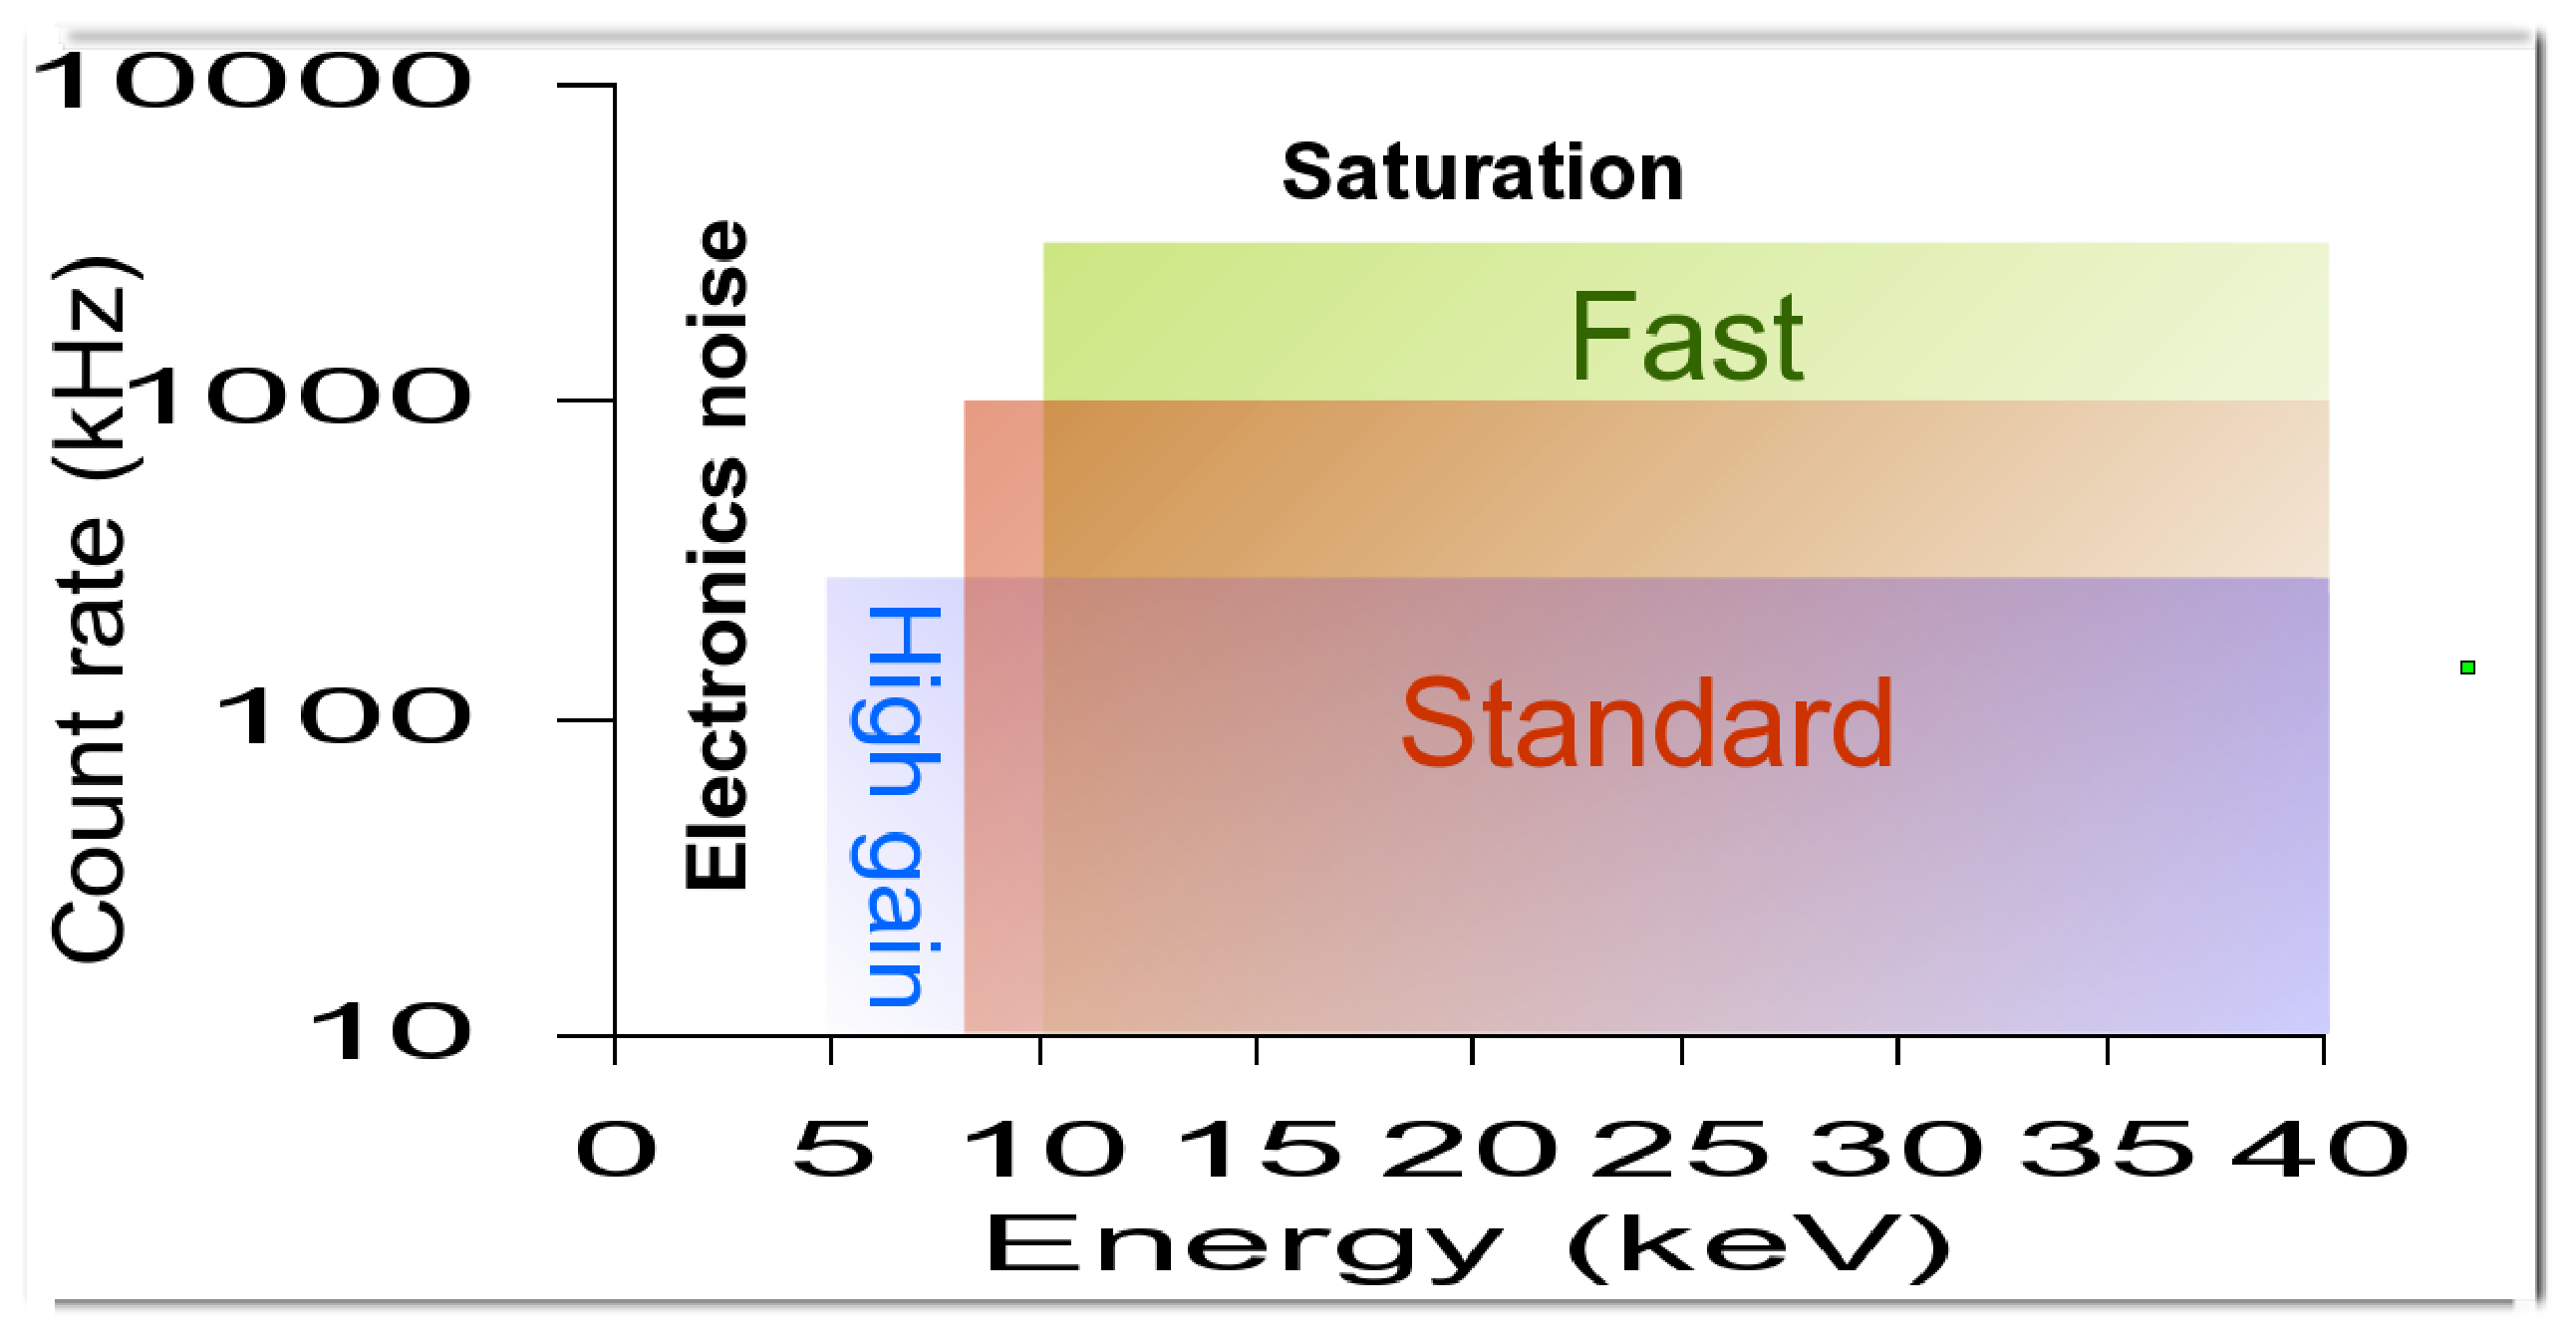
\includegraphics[width=\textwidth]{images/settings}
\end{center}
\caption{Plot indicating the reccomended choice of detector settings as a function of the X-ray energy and maximum count rate per channel..}\label{fig:settings}
\end{figure}


\section{How do I chose the comparator threshold?}

\begin{figure}[b!]
\begin{center}
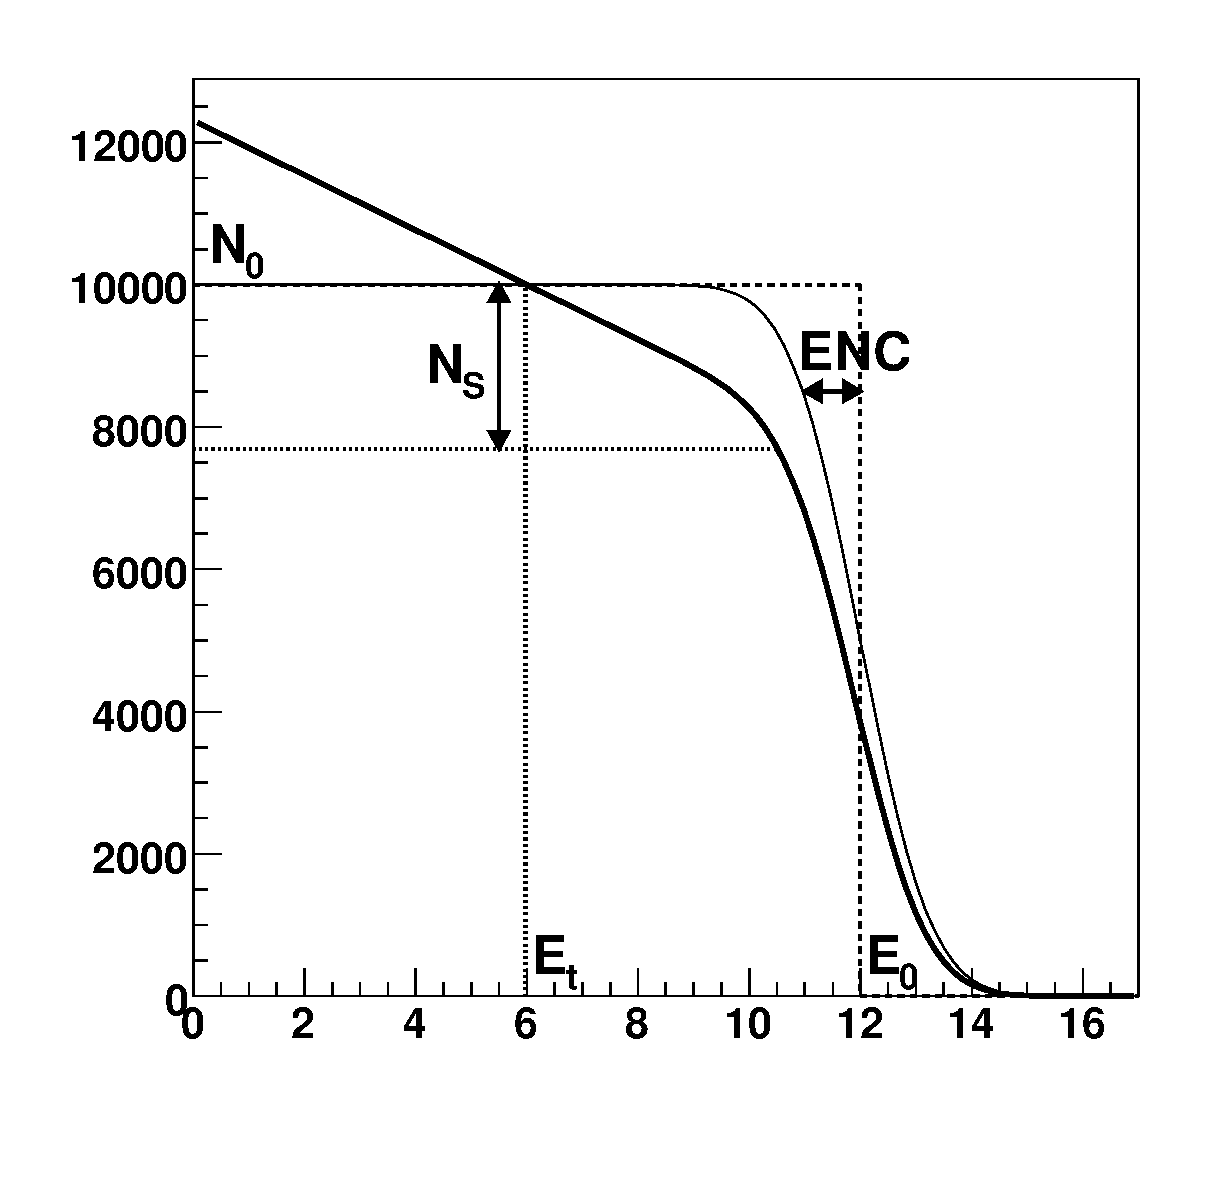
\includegraphics[width=\textwidth]{images/thr_scan_expl}
\end{center}
\caption{Number of counts as a function of the threshold detected in an ideal case.}\label{fig:thrscan}
\end{figure}

\begin{figure}[t!]
\begin{center}
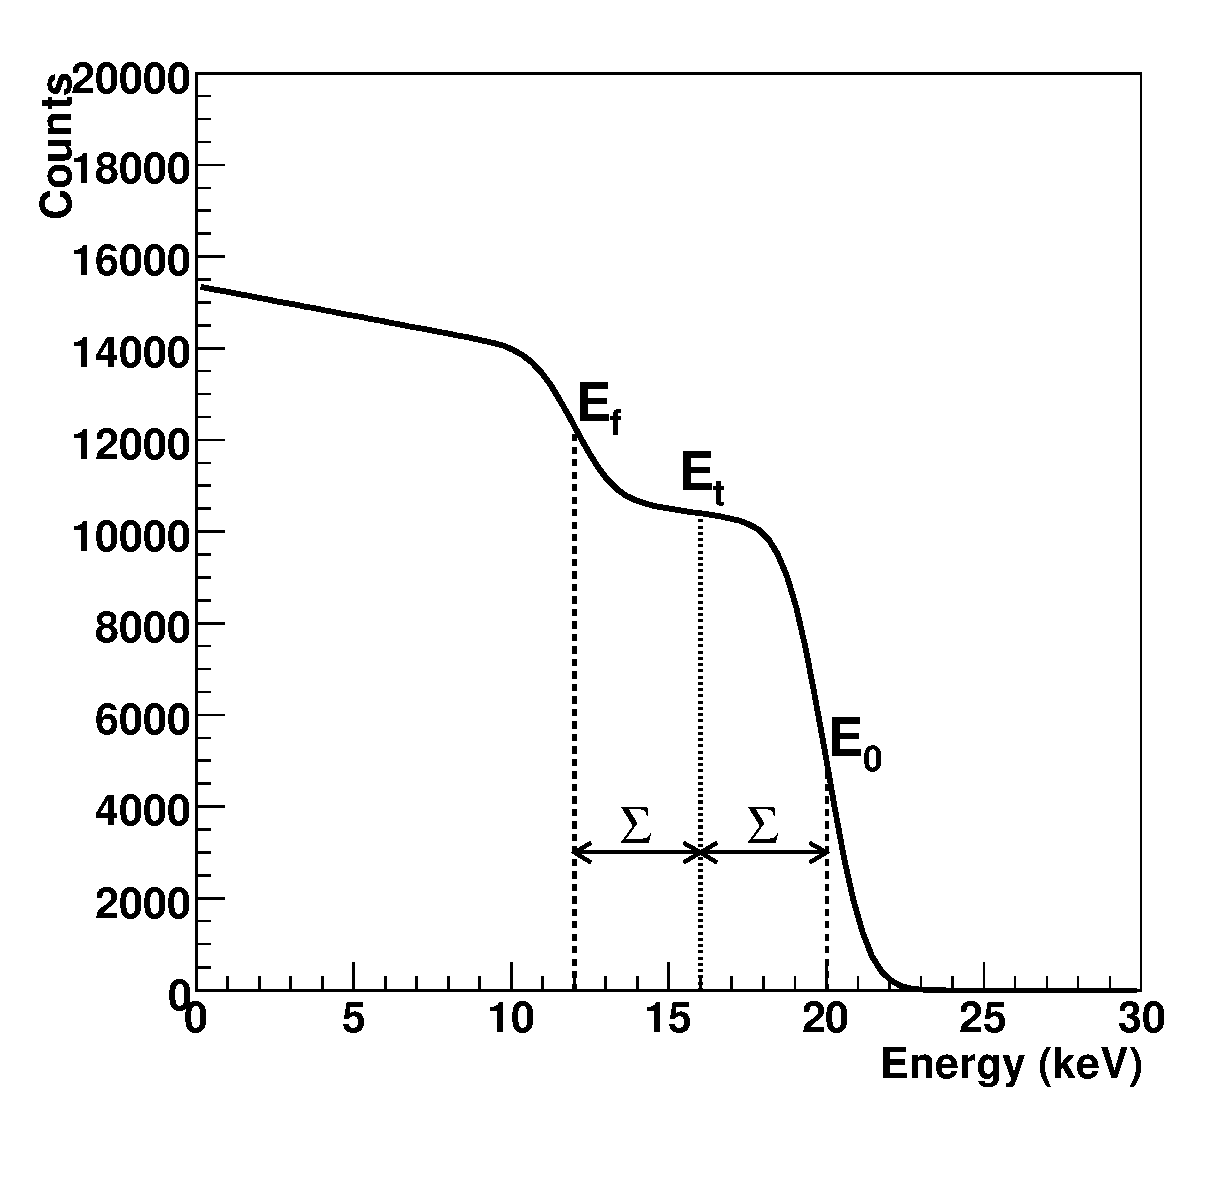
\includegraphics[width=\textwidth]{images/thr_scan_fluo}
\end{center}
\caption{Number of counts as a function of the threshold detected in presence of fluorescent radiation}\label{fig:thrscanfluo}
\end{figure}

Once selected the settings, the threshold should be selected.
Figure~\ref{fig:thrscan} shows the number of counts as a function of the threshold value in the ideal case of monoenergetix X-rays of energy $E_0$=10~keV.
For thresholds larger than the X-ray energy the detector should always count 0 and for lower thresholds it should always count all the photons. However the curve is smoothed around $E_0$ because of the electronic noise (ENC) and is not perfectly flat for lower energies because the photons absorbed in the region between two strips distribute their energy between them and it is not flully collected by a single channel (charge sharing).\\
In order to count once al X-rays the threshold should be set at half of the X-ray energy $E_t=E_0/2$: if the threshold would be higher some photons would not be counted, leading to a loss of efficiency, while if it would be lower some photons would be counted twice leading to a loss of spatial resolution. 

Since the detector threshold can't be precisely set at the same value for all channels but there will always be some spread of the order of 200~eV (threshold dispersion) there will always be some fluctuations on the number of counts between channels, which however should be corrected by the flat field correction.

The choice of the threshold should also depend from  considerations regarding the emission of fluorescent radiation from the sample.\\
Figure~\ref{fig:thrscanfluo} shows  how the curve of the counts would look like for monochromatic X-rays of energy $E_0$ in presence of radiation of energy $E_f$ emitted by the sample. The curve would show a second step at $E_f$. 

Since the fluorecence emission is not present in the flat field data, the difference of counts between the channels due to the fluorescent radiation cannot be corrected and the threshold $E_t$ should be set at an energy larger than $E_f$. This also helps to cut down the background.\\
The difference of counts between the channels will be particularly large if the threshold is set in some ``steep'' part of the curve i.e. close to $E_f$ or to $E_0$ (but in this case it would be corrected by the flat field, at cost of loss of efficiency).
Because of the presence of the electronic noise, $E_t$ should be at least 3~keV larger than $E_f$.

Here is a short list of rules to select the appropriate working threshold in order of importance (and eventually modify the X-ray energy):
\begin{enumerate}
\item List the fluorescent emission lines $E_f$ that you expect from your sample. 
\item If there is no fluorescent emission ($E_f<E_0$) $E_t=E_0/2$
\item If there is fluorescent emission 
\begin{enumerate}
\item $E_t>E_f+3$~keV
\item $E_t<E_0-3$~keV 
\end{enumerate}
If the range where both requirements are satisfied is large, try to increase the distance of $E_t$ from $E_f$ up to 5~keV and then set $E_t$ as close as possible to the ideal value $E_t=E_0/2$
\item If it is not possible to satisfy the previous minimal requirements:
\begin{enumerate}
\item If you need high quality data and you can sacrifice detector efficiency (a lot!)  $E_t>E_f+3$~keV
\item If you need fast measurments and you can sacrifice detector uniformity (difficult to say how much) and increase the background $E_t<E_f-3$~keV. Remember that $E_t$ is klimited by the electronic noise $E_t>4$~keV (3~keV for \textit{High gain} settings).
\item Consider to change $E_0$ to values lower than $E_f$ or at least 6-8~keV larger than $E_f$ 
\end{enumerate}
\end{enumerate}



\begin{figure}
\begin{center}
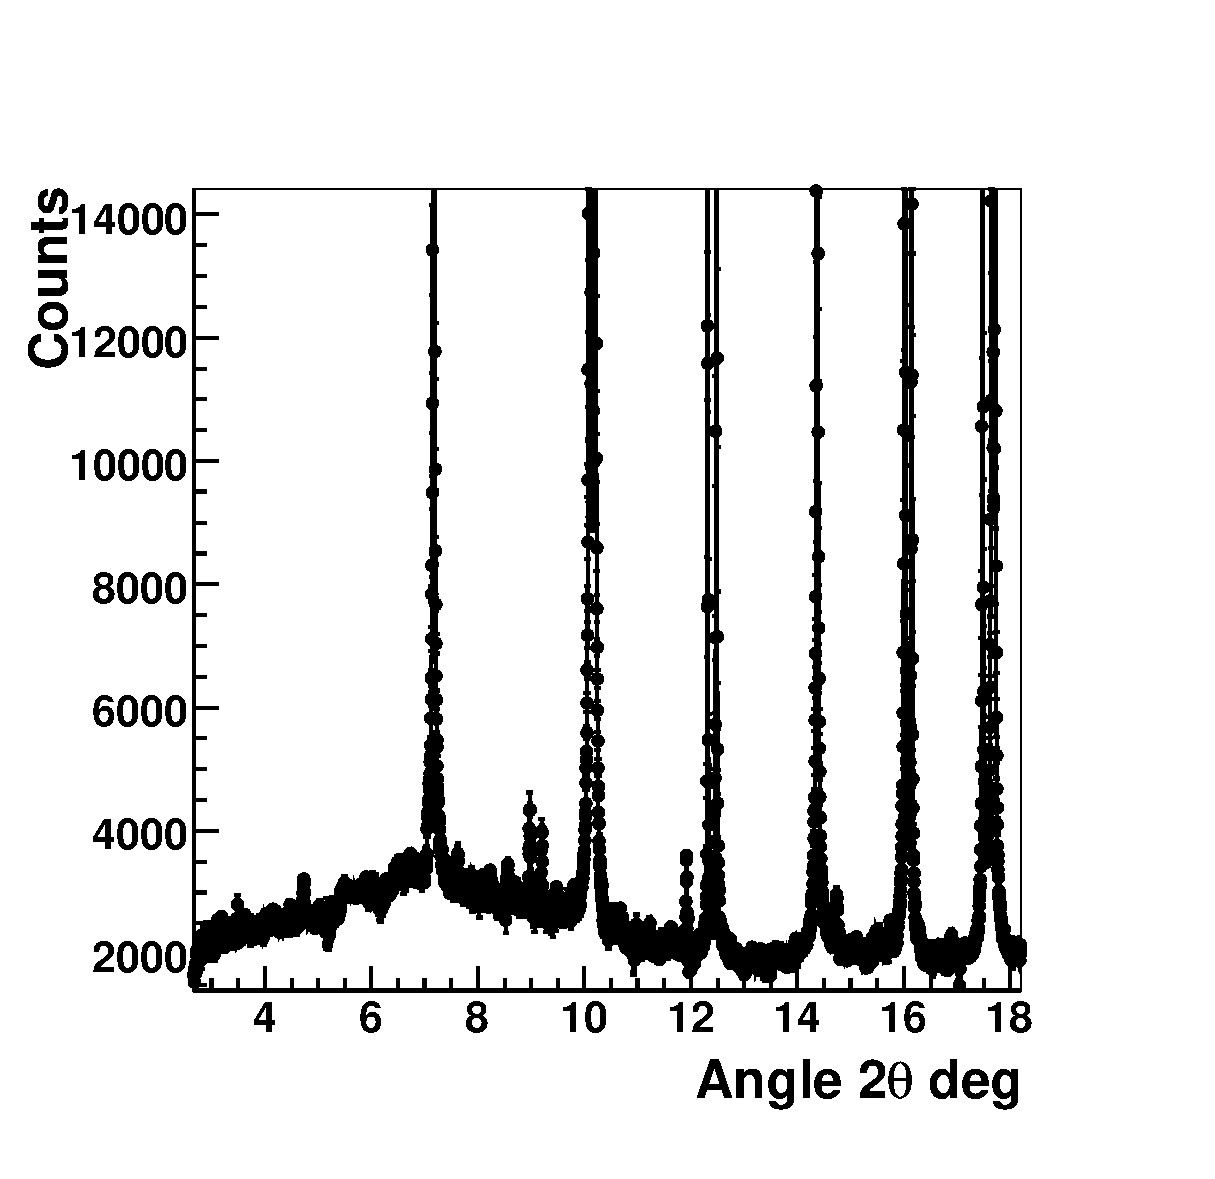
\includegraphics[width=\textwidth]{images/sample_with_fluorescence}
\end{center}
\caption{Example of data from a sample emitting fluorescent light and detector threshold set at a value close to the emission line. The background data cannot be properly flat field corrected.}\label{fig:samplefluo}
\end{figure}


\section{Why isn't my flat-field flat?}

The main reasons of a non flat flat-field can be:
\begin{itemize}
\item The scattering from the glass rod is not uniform over the angular range. In this case you should take the flat field dynamically i.e. scanning the detector in front of the cylinder with the small window, as we do at the SLS. In this case when you shift the detector, the shape of the illumination remains in the same angular position (and shifts in channel number). Of course it depends a lot on the energy and on the geometry of the flat field acquisition.
\begin{figure}
\begin{center}
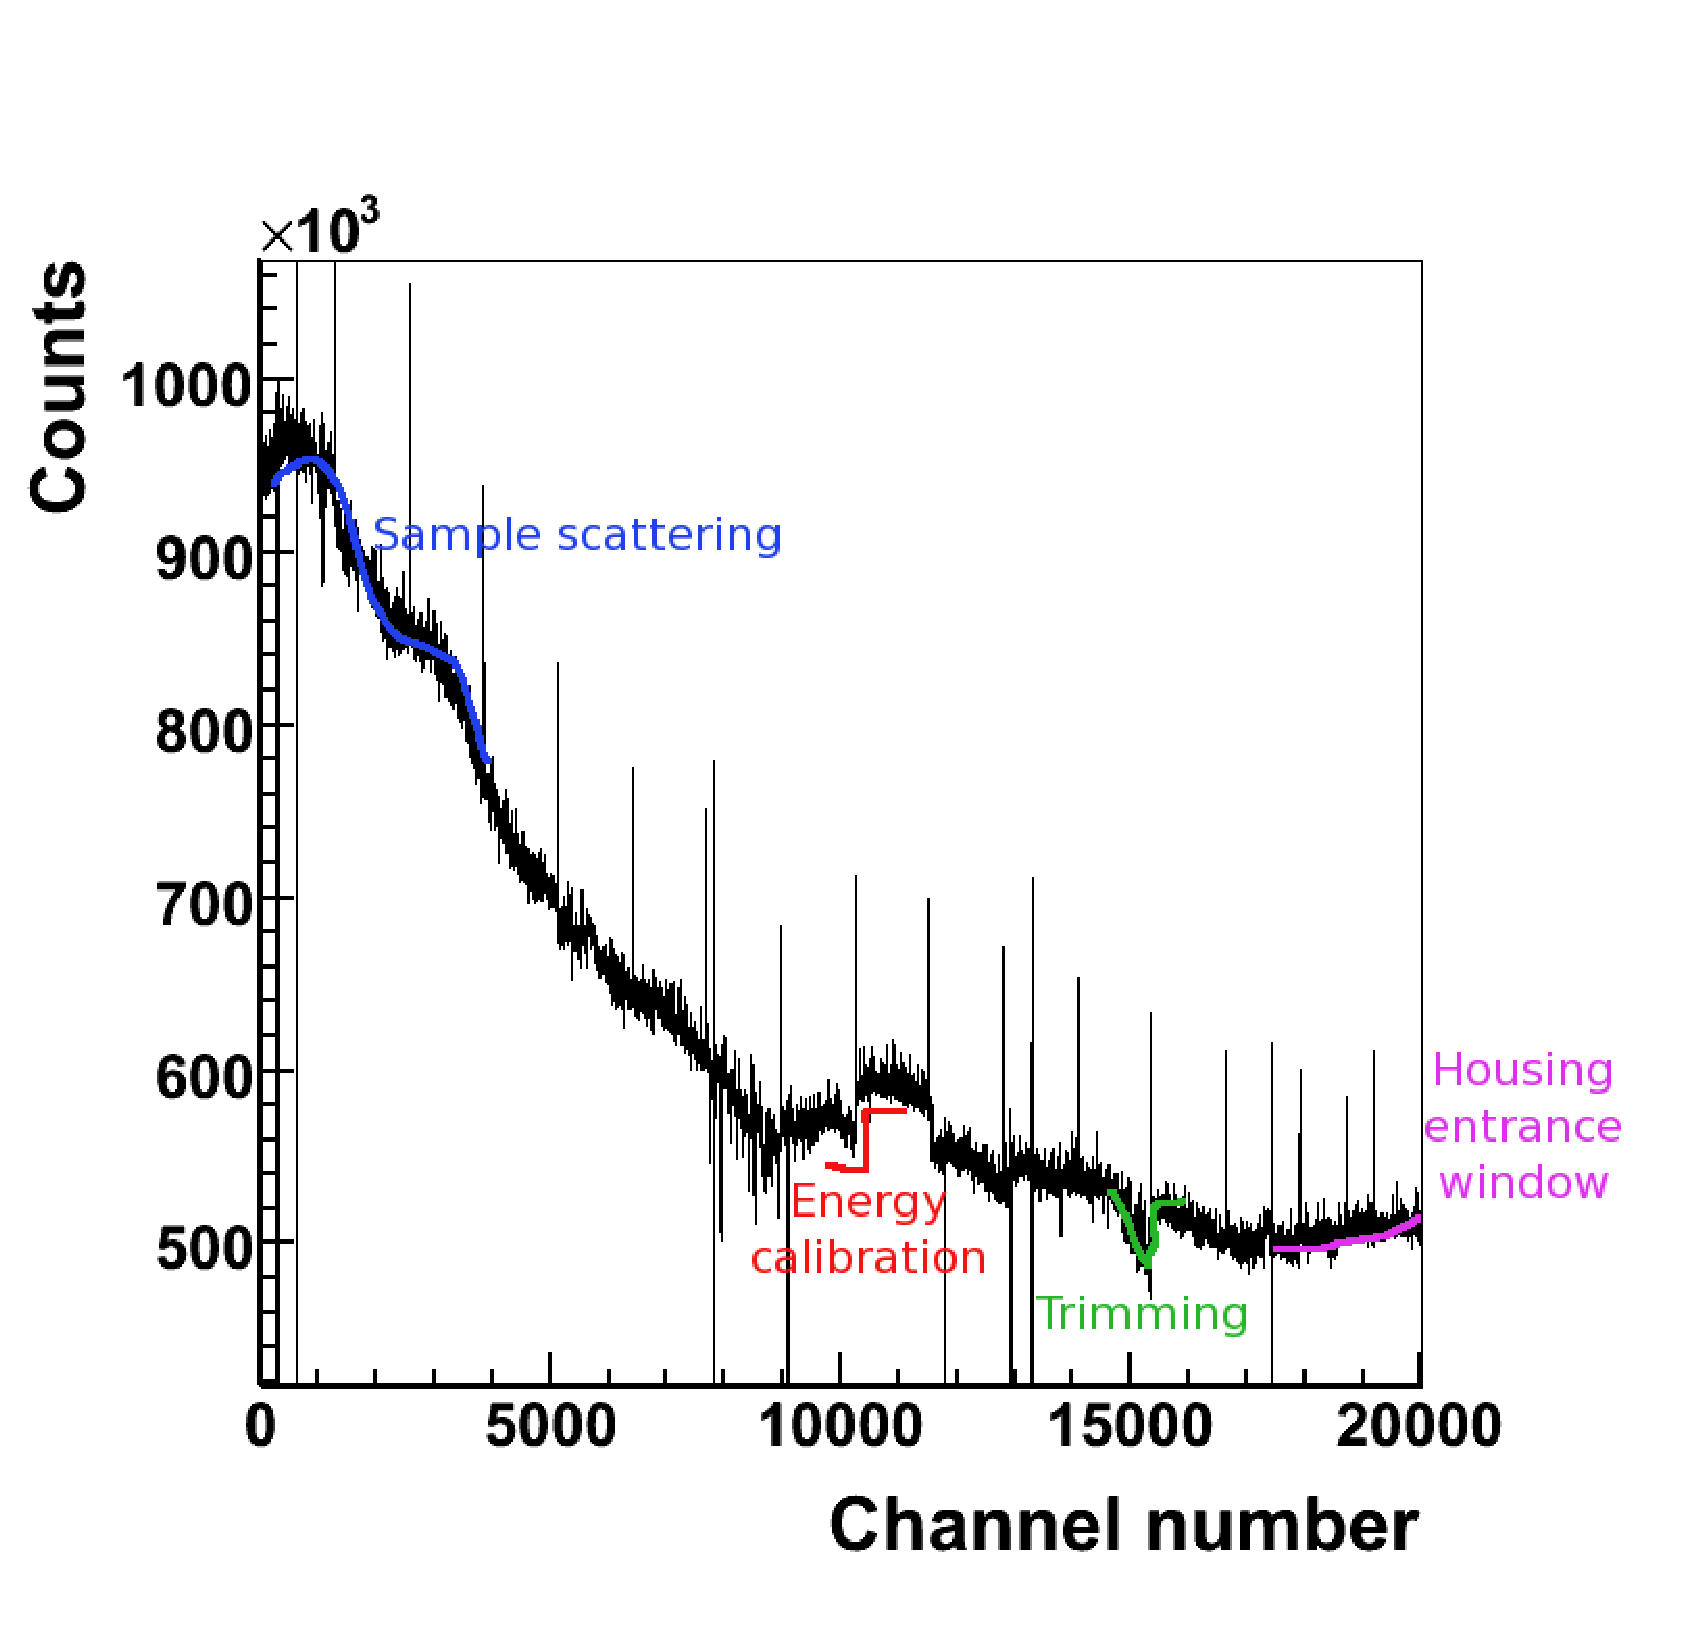
\includegraphics[width=\textwidth]{images/bad_ff_col}
\end{center}
\caption{Example of a very bad flat field data set with highlights of some of the reasons which can cause the non-flat behavior.}\label{fig:badff}
\end{figure}

\item The entrance window for the X-rays is deformed (we also have this problem at the SLS). In this case when you move the detector the "mountain" moves with it in angle (And remains still in channel number). However this should correct without problems with the flat field correction, even in case of fluorescent emission. Should appear at all energies.
\begin{comment}
\begin{figure}
\begin{center}
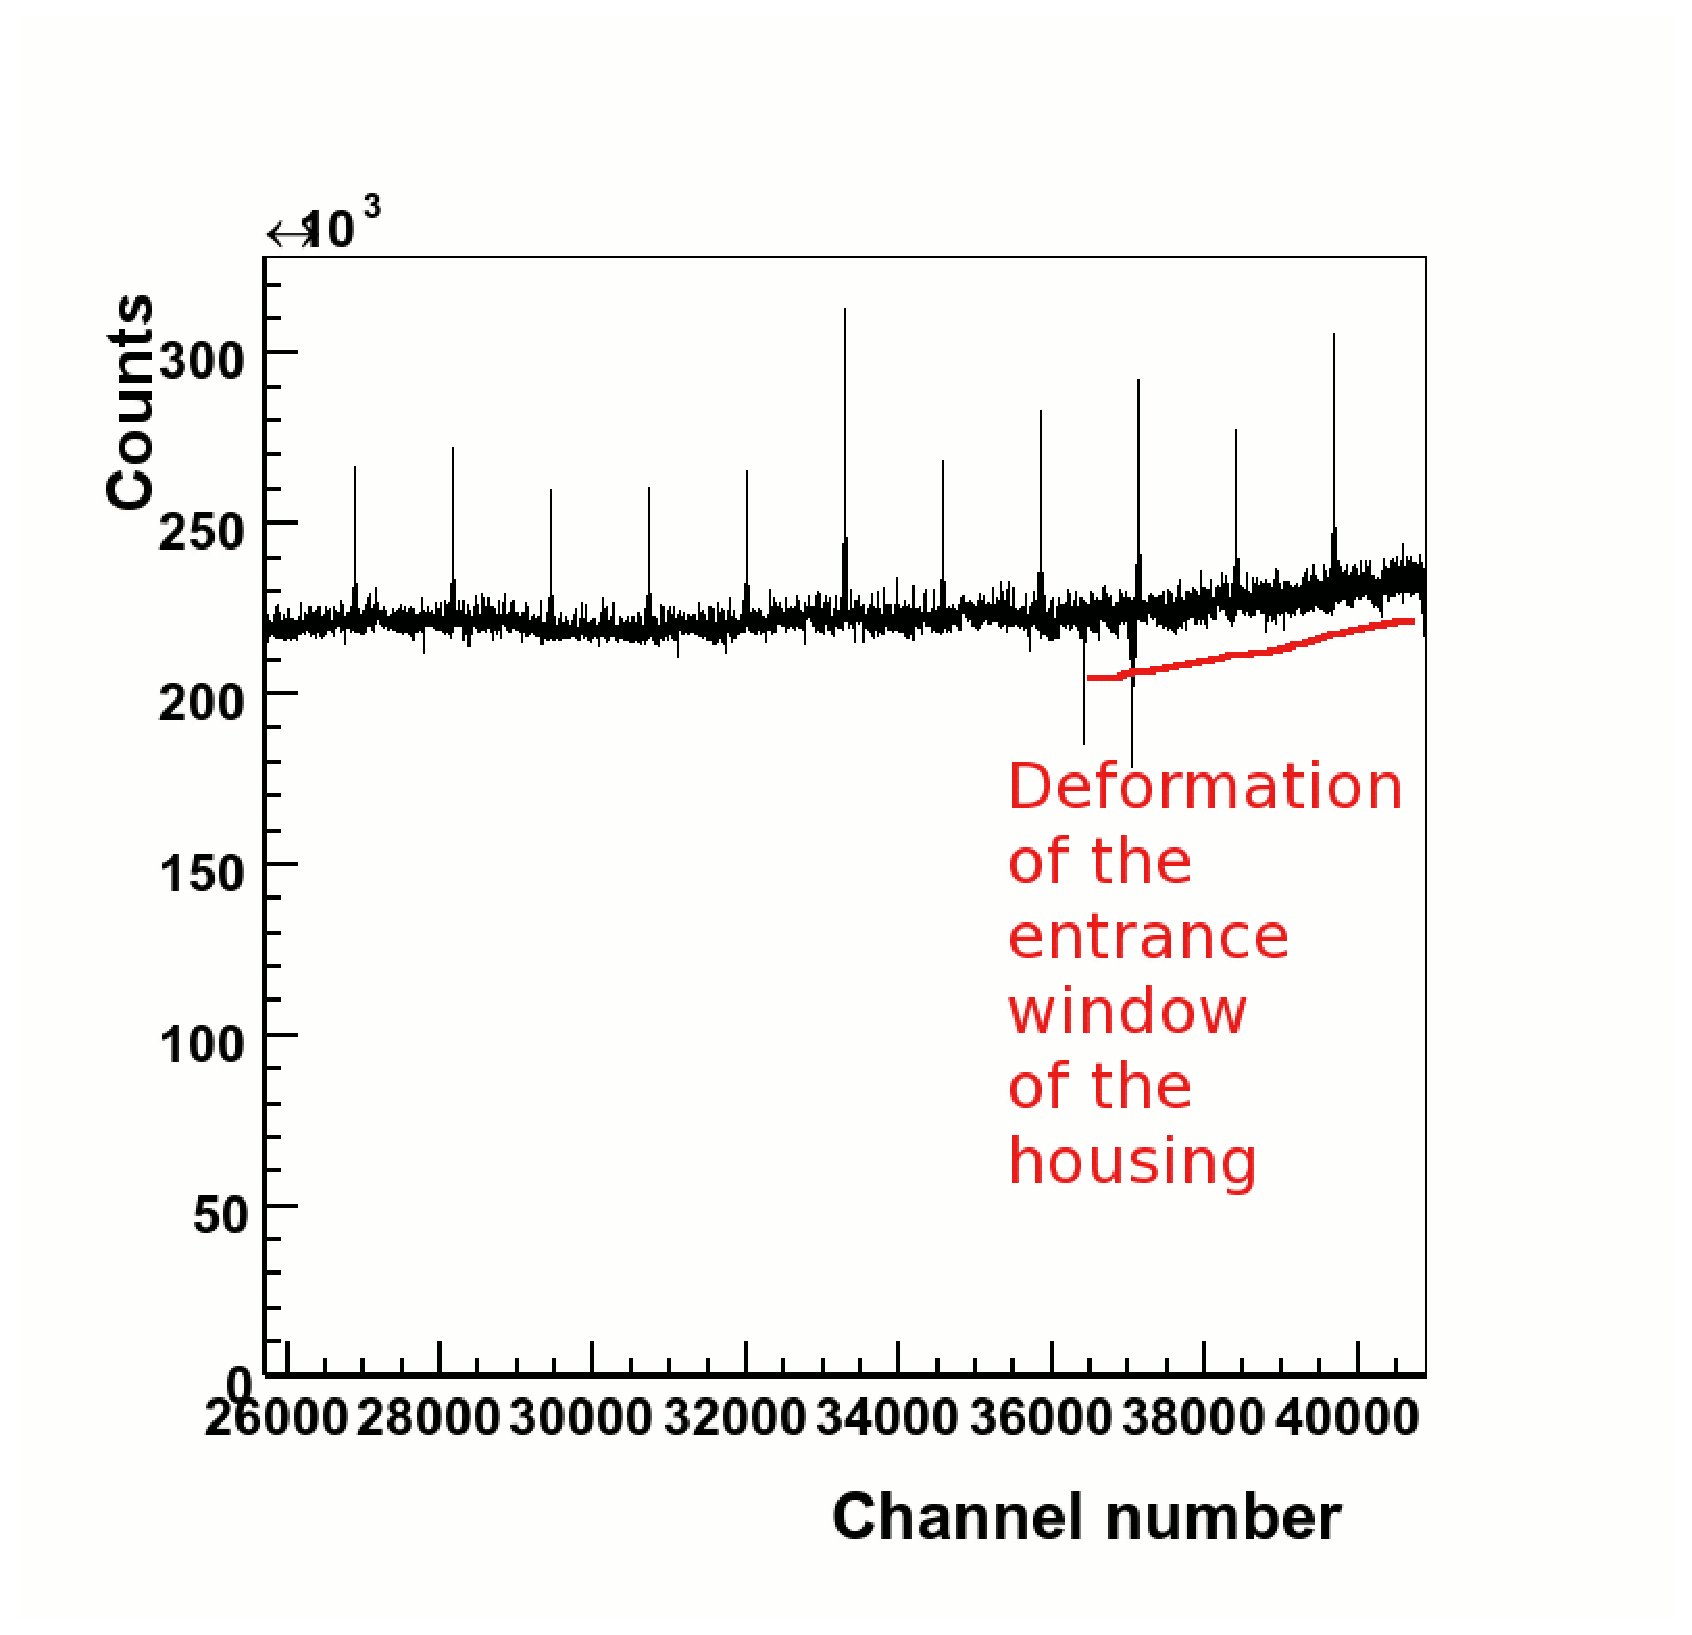
\includegraphics[width=\textwidth]{images/ff_window}
\end{center}
\caption{Variations in the flat field due to a non unifor entrance window of the detector housing.}\label{fig:ffwin}
\end{figure}
\end{comment}
\item Differences of efficiency between the modules i.e. mainly bad energy calibration. You normally see really steps at the transition between modules. Sometimes you have some groups of strips withing a module that are not properly trimmed and look as smallish peaks or valleys in the flat field. When you move the detector, these steps or peaks move in angle and remain still in channel number.
These differences can slightly change as a function of the energy (probably more evident at lower energies) but should normally always be there for the same settings.
These differences get much worse in presence of fluorescent emission, but normally correct properly with flat field correction.
\end{itemize}
\begin{comment}
\begin{figure}
\begin{center}
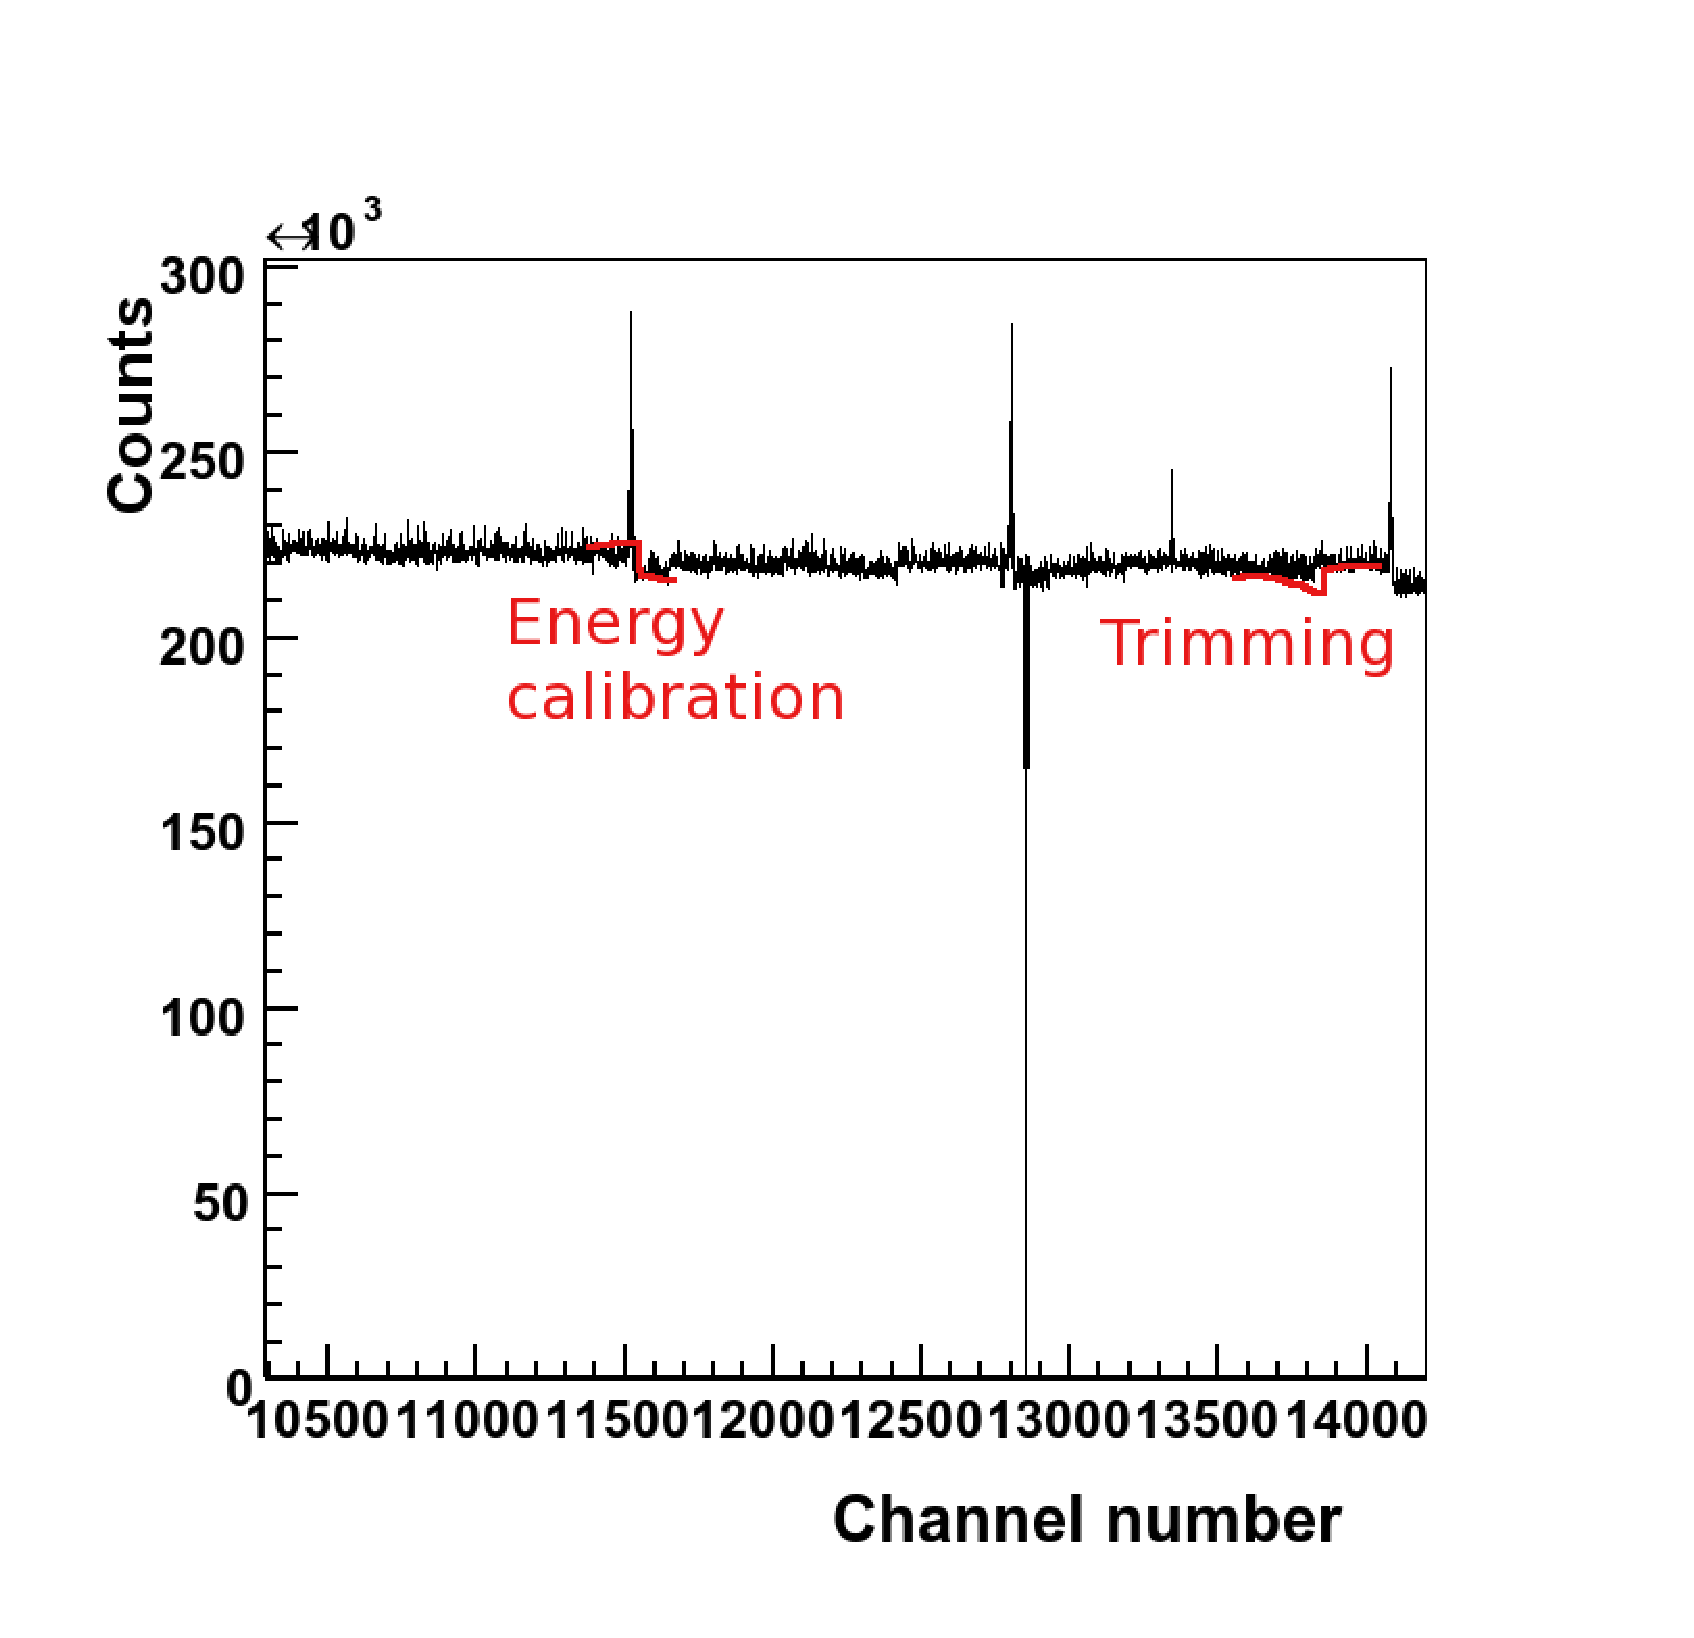
\includegraphics[width=\textwidth]{images/ff_calibration}
\end{center}
\caption{Variations in the flat field due to a non precise energy calibration or trimming of the detector modules.}\label{fig:ffcal}
\end{figure}
\end{comment}
\subsection{Dynamic acquisition of the flat field}

\begin{figure}
\begin{center}
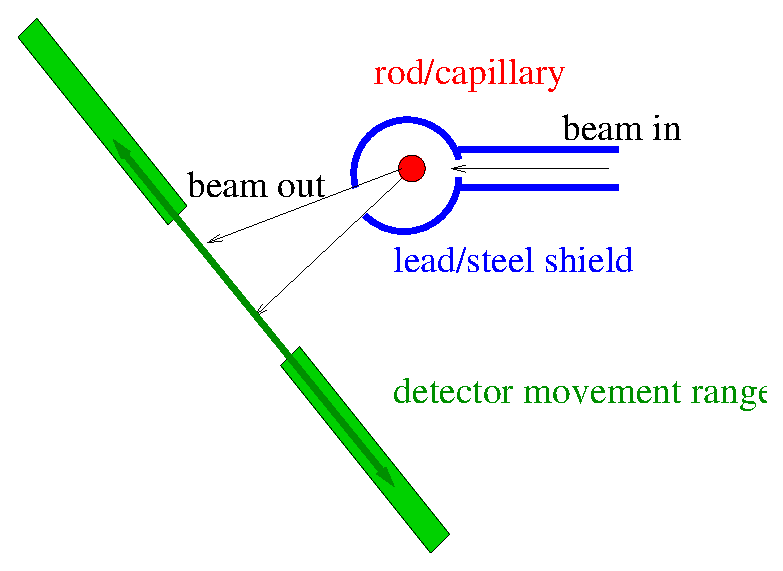
\includegraphics[width=\textwidth]{images/FFSetup}
\end{center}
\caption{Sketch of the experimental setup for a dynamic acquisition of the flat field.}\label{fig:ffsetup}
\end{figure}

\section{What happens when I trim the detector?}

General remarks about trimming.

\subsection{MYTHEN}

%\subsubsubsection{Trimming with noise} \label{sec:noisetrim}
\textbf{Trimming with noise} \label{sec:noisetrim}\\

The first step in the trimming procedure is to trim with noise (this is often sufficient). This has to be done for all the settings which are foreseen to be used (highgain, standard and fast).\\
The procedure for the noise trimming is as follows:
\begin{enumerate}
\item In the \textit{Initialization tab} click on the settings for which you want to trim (e.g. standard)
\item In the \textit{Initialization tab} click on the \textit{advanced} radio button to make the trimming accessible.
\item  In the \textit{Acquisition tab} set the acquisition time to 100~ms, the repetion to 1 and the delay between frames to 0.
\item For noise trimming usually the default parameters $Vthreshold=7$, $Counts=500$, $Resolution=4$ work.\\
However, to verify the threshold setting it is best to make a threshold scan. To do this go to the \textit{Data} tab, in the Data display section select the 2D color and type advanced option. In the \textit{Acquisition} tab select your data directory. Set the number of positions to 0. Select Scan, Type threshold. Typical values for the range are 500 to 900 with a step size of 10. Then click on the start button to perform the threshold scan. After the threhold scan has finished an image similar to the one in~\ref{fig:thresholdscanuntrimmed} should be shown. Depending on the system the number of modules may vary. If the plot is similar to the one in~\ref{fig:thresholdscantrimmed} the noise trim files did already exist and have been loaded when selecting the settings. In this case you don't need to trim with noise again.\\
Set the parameter Vthreshold in the \textit{Trimming} box (\textit{Initialization tab}) 10-30 DAC units below the onset of the noise for the module with the lowest threshold offset. Since the modules have differences in the offset and gain the onset of the noise varies. \\
You can usually leave the remaining parameters unchanged (Counts/pixel=500; Resolution=4).
\item Select the directory where the noise trim files should be written and the filename, to wich will be attached the extension given by the module serial number (.snxxx). If you want the trimfiles to be loaded authomatically when the global settings are selected, select the default directory specified in the config file (or in the ``trimbits/beamline'' directory for the older software versions). 
Click on \textit{Trim} to start the noise trimming process. After the trimming has finished look at the plot and the distribution of the trim bits. The distribution should be around 32$\pm$5 and should look gaussian. An example distribution is shown in figure~\ref{fig:trimdistribution} and an example plot in~\ref{fig:trimplot}. If the distribution is too much off center change the counts/pixel, if it is too narrow reduce the resolution (set it to 3), if it is too wide increase it (set it to 5). Make sure not too many channels have a trim value of 0 or 63.
\item Execute the treshold scan again to verify the trimming was done properly. A plot similar tho the one in figure~\ref{fig:thresholdscantrimmed} should appear.
\end{enumerate}

\begin{figure}
\begin{center}
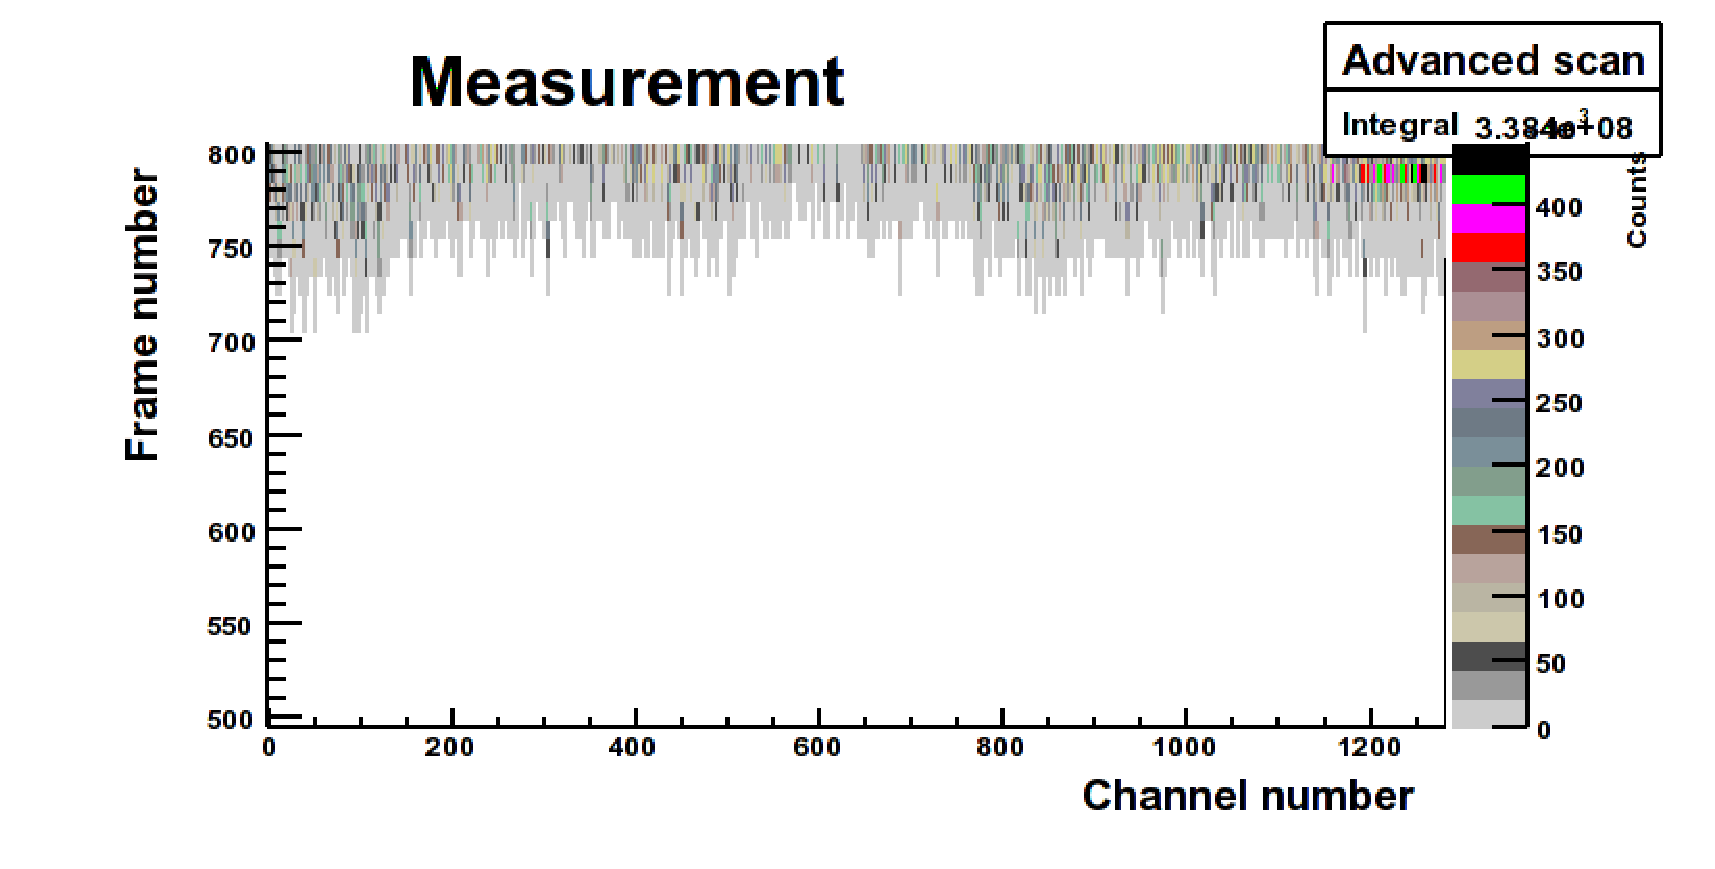
\includegraphics[width=\textwidth]{images/noise_thresholdscanuntrimmed}
\end{center}
\caption{The untrimmed threshold scan.}\label{fig:thresholdscanuntrimmed}
\end{figure}

\begin{figure}
\begin{center}
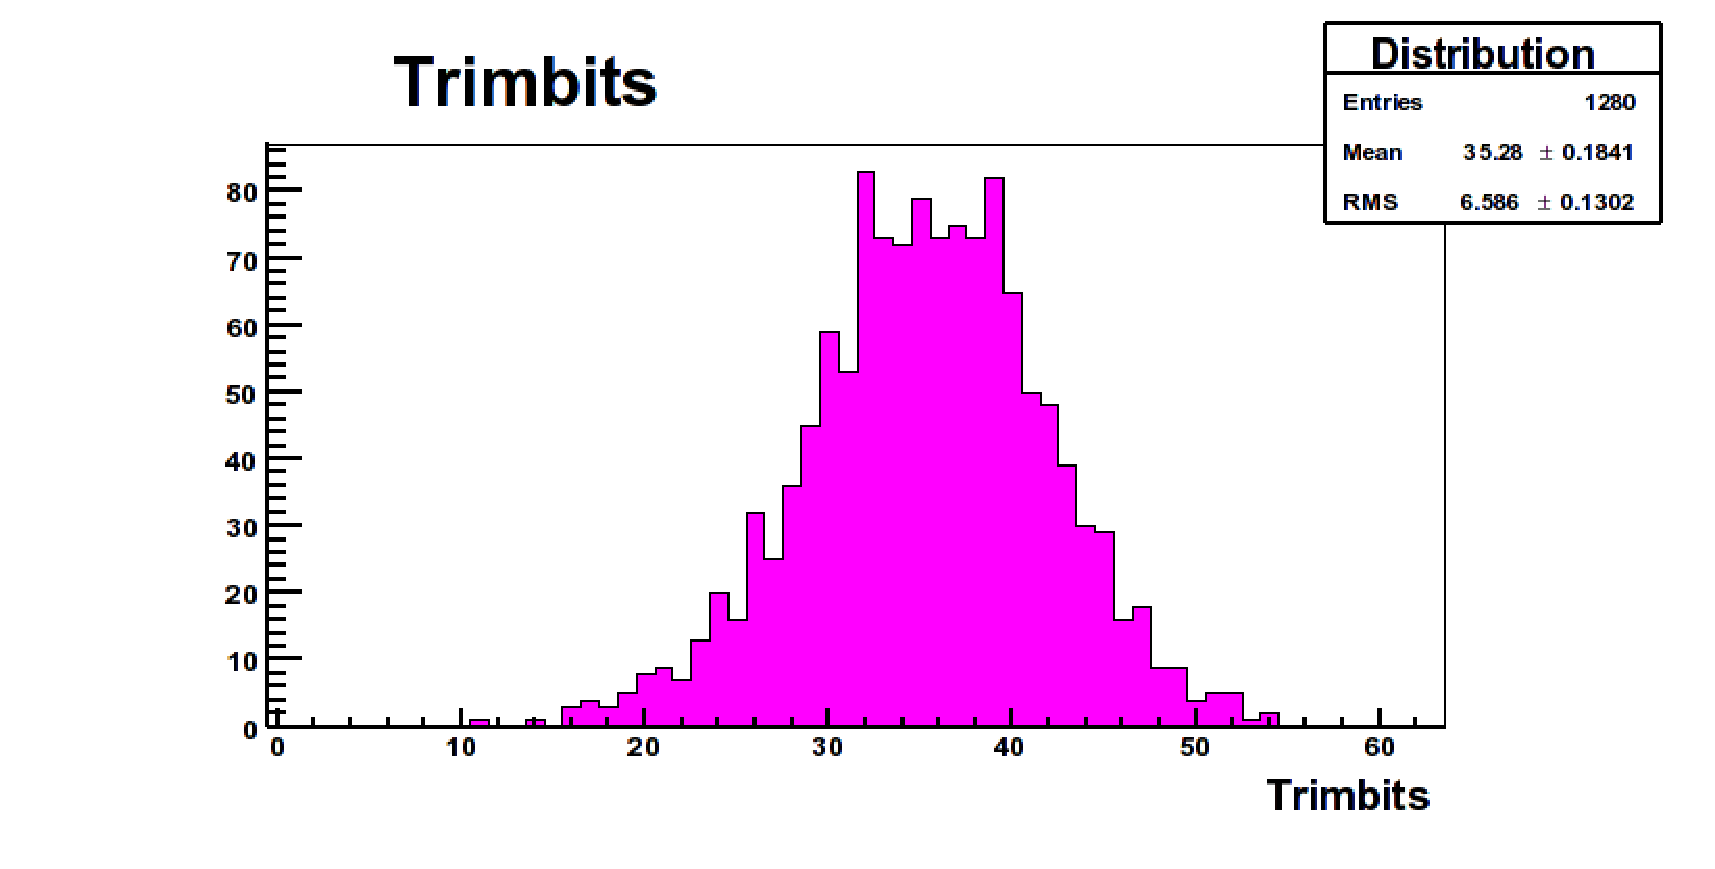
\includegraphics[width=\textwidth]{images/trimbitdistribution}
\end{center}
\caption{The distribution of the trimbits.}\label{fig:trimdistribution}
\end{figure}

\begin{figure}
\begin{center}
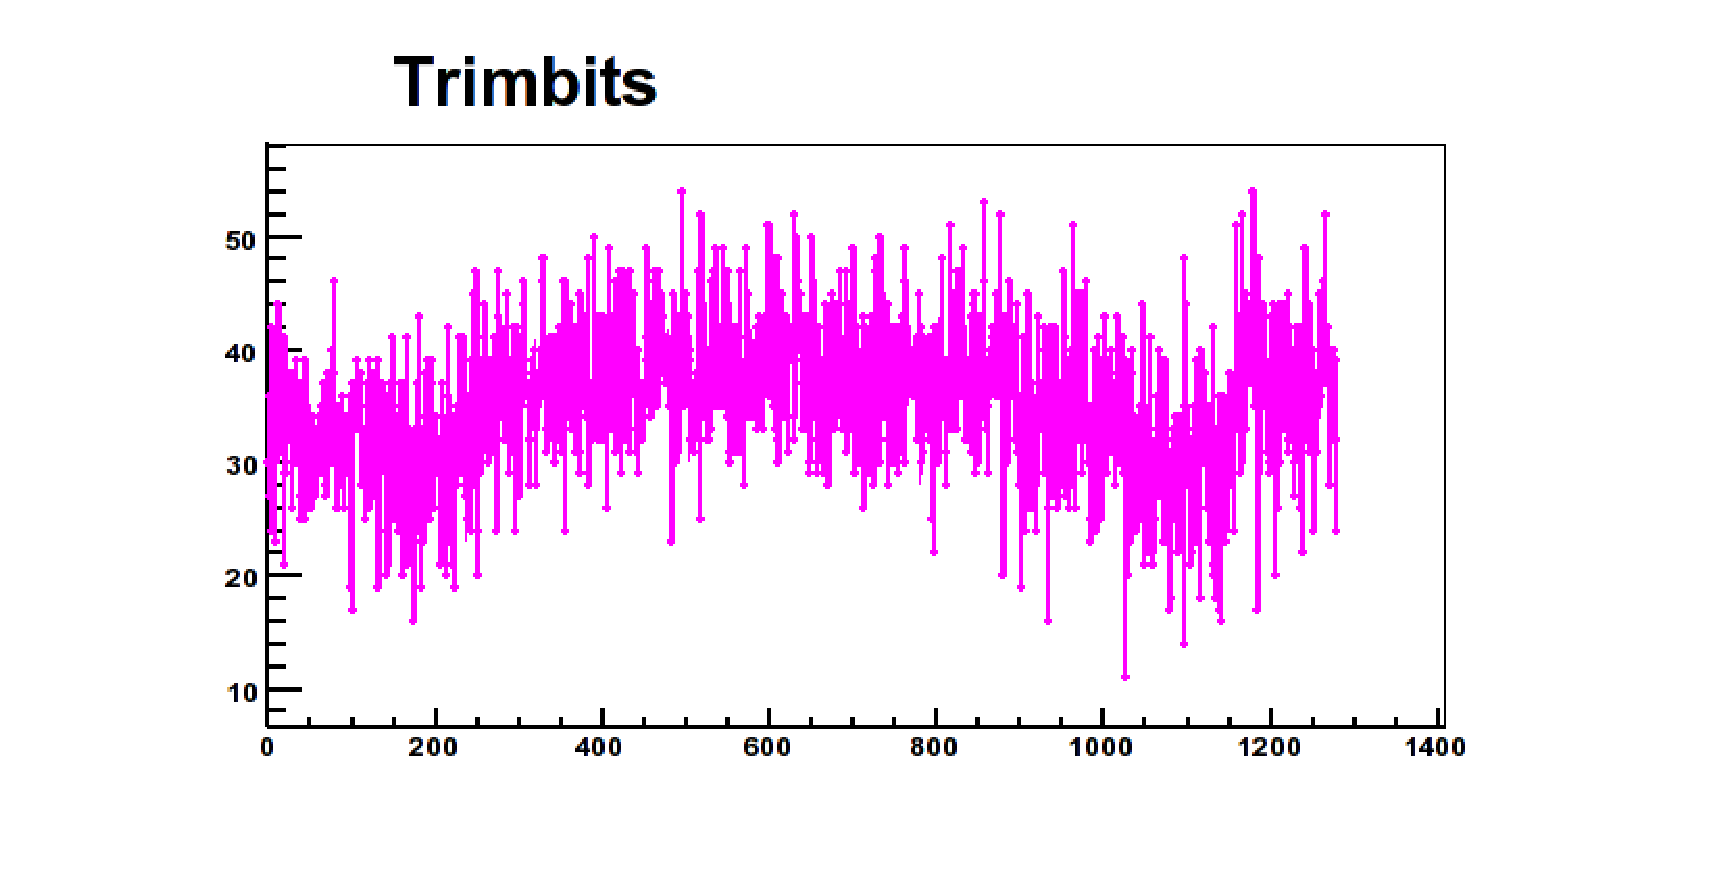
\includegraphics[width=\textwidth]{images/trimbitplot}
\end{center}
\caption{The trimbits for all the channels.}\label{fig:trimplot}
\end{figure}

\begin{figure}
\begin{center}
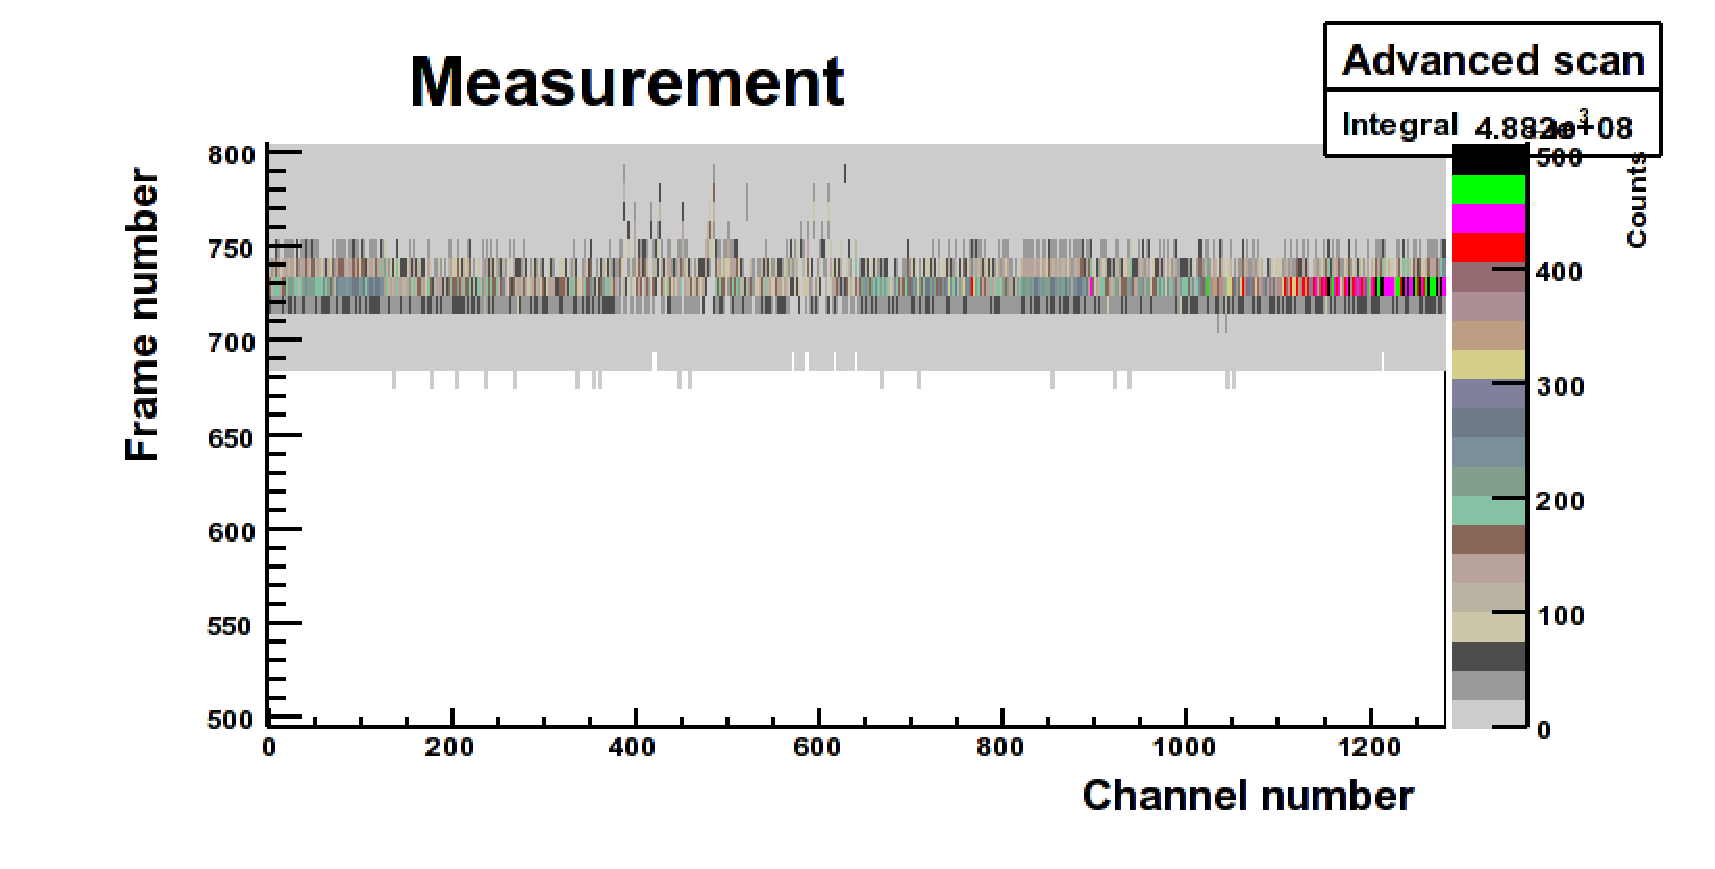
\includegraphics[width=\textwidth]{images/noise_thresholdscantrimmed}
\end{center}
\caption{The trimmed threshold scan.}\label{fig:thresholdscantrimmed}
\end{figure}
\textbf{
%\subsubsubsection{
Improve the trimming using X-rays}\label{sec:improvetrimming}\\

The improvement of the trimming acquired with noise is not essential: at 12~keV an untrimmed module has a threshold dispersion which is about 1.4~keV and is already reduced to 200~eV at 12~keV by the noise trimming. At lower energies the noise trimming will be more effective, while the threshold dispesion will be still larger at higher energies. The trimming improvement reduces the threshold dispersion to 140~eV at 12~keV and is expected to be almost constant at all energies. For this reason it is suggested to perform the trimming improvement only when a small threshold dispersion is really important (e.g. to avoid flat field corrections or in presence of fluorescent lines close to the threshold value) and it will probably be not worthy at lower energies (i.e. threshold lower than 6~keV and X-ray energy lower than 12~keV). 
The procedure for the trimming improvement is as follows:
\begin{enumerate}
\item Select the settings of the detector and load the noise trimming file
\item Set the threshold at half of the X-ray energy (better if the detector has already been calibrated in energy like explained in~\ref{sec:encal})
\item Illuminate the detector with a flat field. This is very important to obtain a good trimming. 
\item Select the \textit{acquisition time} in the \textit{acquisition tab} so that there are at least 1000 counts/strip per frame (the more counts, the better trimming). Set the repetions to 1 and the delay between frames to 0.
\item Go to expert mode by clicking on \textit{advanced} in the \textit{initialization tab}, \textit{settings} box
\item In the trimming box  select the directory where the noise trim files should be written and the filename, to wich will be attached the extension given by the module serial number (.snxxx).
\item Select the \textit{improve} method
\textit Start the trimming
\end{enumerate}
If the trimming is correctly performed and the illumination is flat enough, the same trimming can be used every time you will measure at this same energy.
The authomatic loading of energy-specific trim files is not yet implemented.

\section{In what consists the energy calibration of the detector?}\label{sec:encal}

General remarks about DAC to energy conversion

\subsection{MYTHEN}

Since the conversion between the threshold DAC units and energy depends on the gain and offset of the channels the energy calibration has to be done for all settings (high gain, standard and fast). For each setting follow this procedure:
\begin{itemize}
\item Select the setting in the \textit{Initialization} tab.
\item Enter in expert mode by clicking the \textit{Advanced} radiobutton in the \textit{Global settings} box in the \textit{Initialization} tab.
\item If the trimfiles are in the correct location and with the correct name, they should be loaded by default every time you select the corresponding settings in the \textit{global settings} box in the \textit{initialization} tab~\footnote{The default name of the calibrated trimfiles is \textsf{trimbits/beamline/}\textit{settings}\textsf{/noise.snxxx} where  \textit{settings} is the chosen settings. You  can change it in \textsf{src/qDetector.h} and then recompile the acquisition program as described in~\ref{sec:installation}.}.
If the trim files do not yet exist generate them as explained in section~\ref{sec:noisetrim}.
\item Execute a threshold scan of the detector with at least three different energies. The more monochromatic are the X-rays, the better the calibration will be (i.e. scattered X-rays are better than the fluorescent emission). \\
The scan should range from where all modules count 0 (estimate 850-20$\cdot$energy(keV) DAcu) and where all modules start having a lot of noise (usually 800 DACu) with a step of 1 or 2 DACu. The acquisition time should be chosen so that there are at least 1000 counts per strip on the plateau.
\item Open the file \textsf{root/CalAllModules.C} for editing. Change the value of the following global variables according to your needs:
\begin{itemize}
\item \textit{nmod} is the number of modules of your system.
\item \textit{nscan} is the number of different threshold scans you acquired.
\item \textit{en} is the array with the energies at which you acquired the scans, in keV.
\item \textit{een} is the array with the errors on the energies at which you acquired the scans, in keV. It is usually small, but can be some hundreds eV in case of dirty fluorescent samples.
\item \textit{fn} is the array containing the location and root file name of your data.
\item \textit{run} is the array containing the run index of your data.
\item \textit{startscan} is the array containing the threshold value at which you started the scans.
\item \textit{stopscan} is the array containing the threshold value at which you finished the scans.
\item \textit{stepscan} is the array containing the threshold step of the scans.
\item \textit{ave} is the array containing the average number of counts per strip on the plateau (it must not be too precise).
\item \textit{sn} is the array containing the list of the serial number of the modules to be calibrated. It is important that the list is in the right order, so that the optput calibration files have the extension .snxxx corresponding to the right module.
\item \textit{of} is the location and root file name of the calibration file. The directory should already exist and the extension .snxxx will be attached to the output file.  
\end{itemize}
\item Launch \textsf{root}, which you should have already installed on your linux PC
\item Execute the following commands in order to load the macros needed for the calibration:
\begin{verbatim}
root$ .L root/NewMythenMacros.C++
root$ .L root/CalAllModules.C++
\end{verbatim}
You should get a lot of warnings, but no errors.
\item Execute the following command in order to run the calibration:
\begin{verbatim}
root$ EnCalModules()
root$
\end{verbatim}
Reading and analyzing the data takes some time, but, after a while, a canvas should open where the plots of the median of the counts of every module as a function of the threshold should be shown for each energy, fitted with a modified \textit{erf} function in order to find the inflextion point. The last plot of the canvas should represent the inflexion points as a function of the energies, and by fitting it with a straight line it is possible to calculate the offset and gain for each module i.e. calibrate it as a function of the energy. Please check that this automated fitting procedure succeeds. In case you see many fitting errors you should try to check wether the variable you edited in  \textsf{root/CalAllModules.C} are all correct or try to edit the fitting procedures in the two root macro files (sorry!).
\item Copy the calibration file you obtained to \textsf{calibration}/\textit{settings}\textsf{.snxxx}~\footnote{The default name of the calibration file \textsf{calibration/}\textit{settings}\textsf{.snxxx} where  \textit{settings} is the chosen settings. You  can change it in \textsf{src/qDetector.h} and then recompile the acquisition program.} By doing this the correct threshold for each module will be calculated every time you change the \textit{threhsold energy} in the \textit{global settings} box in the \textit{initialization} tab, you have loaded some default settings and you are not in expert mode.  
\end{itemize}

\section{Why should I change the dynamic range of the counters?}

\section{When should I enable rate correction}
\subsection{How can I choose the dead time?}





%\begin{comment}
\chapter{Charge Integrating detectors}

Various issues concerning calibration, dynamic gain switching, data handling data processing etc.
\section{(Dynamic) Gain Switching}
\section{Pedestals}
\section{Energy calibration}
\section{Data processing}





\chapter{Angular conversion}


\section{How is the channel number coverted into angle?}\label{sec:angcal}


%\begin{figure}[!h]
%\centering 
%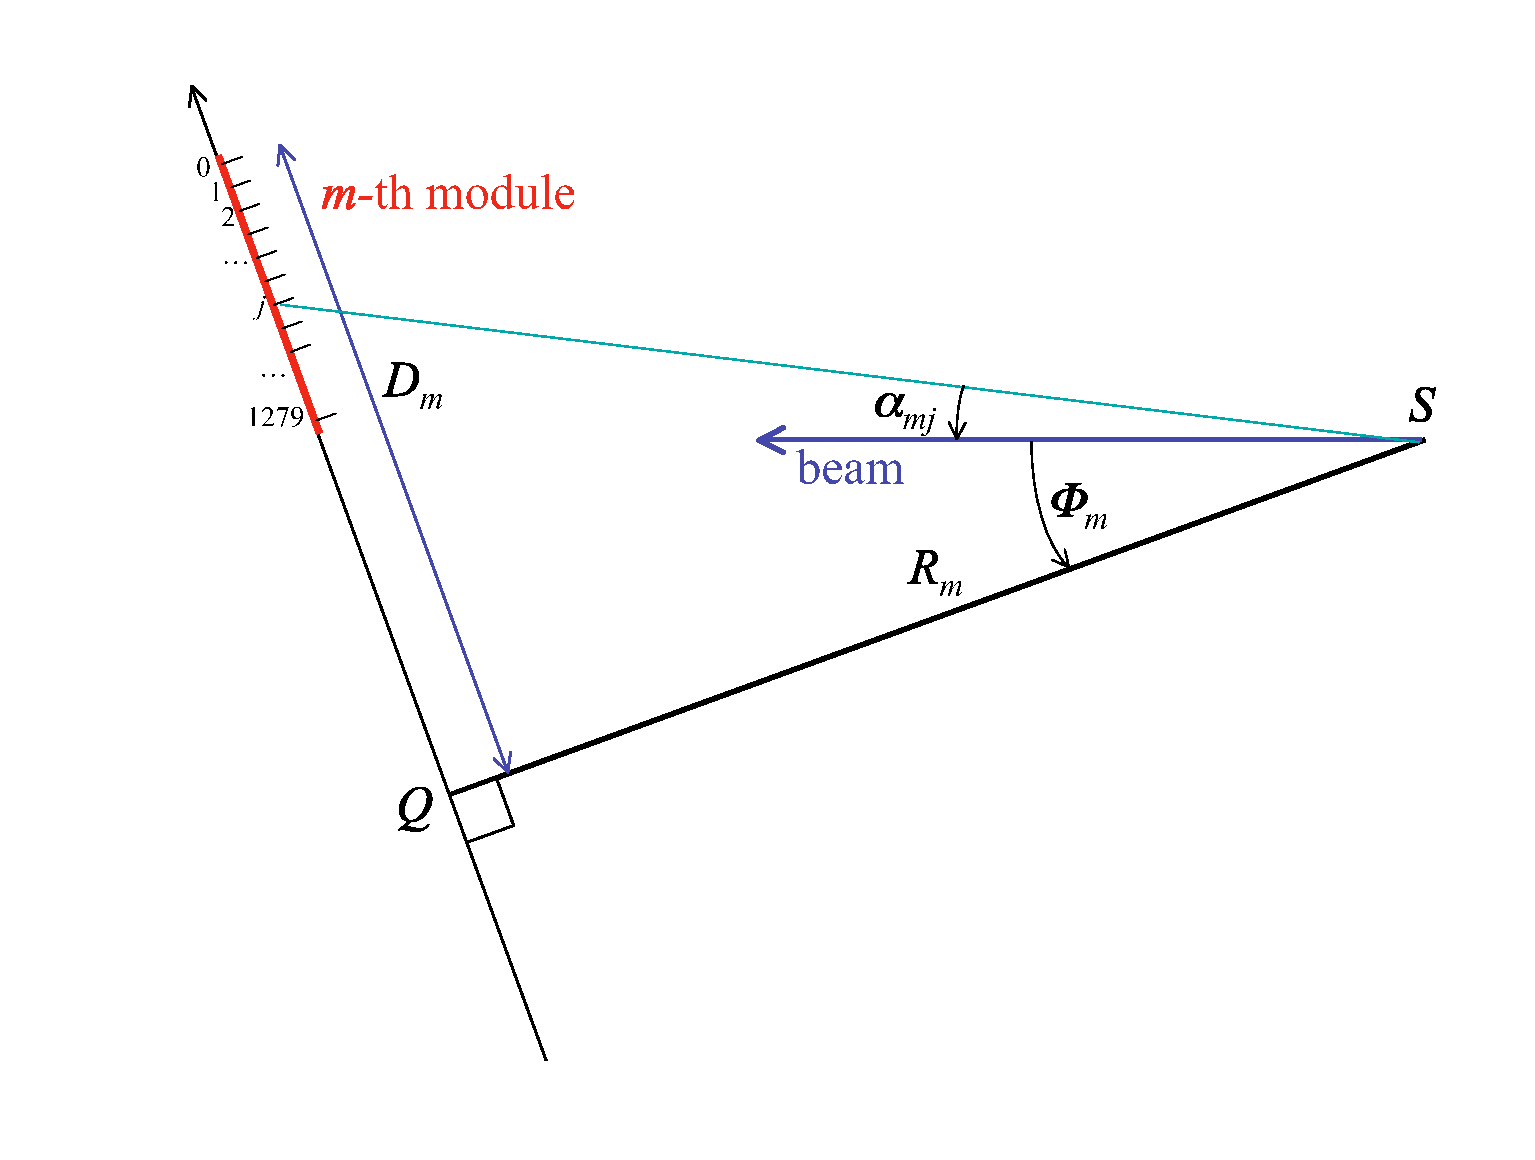
\includegraphics[width=0.98\textwidth]{AngConv}
%\caption{Schematics of the scattering geometry in the diffraction plane. A Mythen II module is shown. $R_m$ is the distance from the module sensor plane (orthogonal to the diffraction plane) to the sample position $S$; $D_m$ the distance from the center of pixel $j=0$ to point $Q$, counted positively as the arrow on the module plane goes (\emph{i.e.}, oppositely to the direction of increasing $j$); $\Phi_m$ is the angle of the module plane normal with the beam direction, positive counterclockwise. $\alpha_{jm}$ is the angular position of the $j$-th pixel center with respect to the beam direction, positive counterclockwise.}
%\label{acon}
%\end{figure}

Mythen II modules are composed by 1280 pixels, each having width p=0.05~mm, and numbered with j=0,..,1279. 
Angles are counted counterclockwise from the beam direction. For the m-th module, the angle $\alpha_{jm}$ of its j-th pixel center 
can be determined using the three geometric parameters $R_m$~[mm], $\Phi_m$~[deg], $D_m$~[mm], as in \fref{acon}. 
The detector group uses instead the 3 parameters center $c_m$~[\ ], offset $o_m$~[deg], conversion $k_m$~[\ ]. 
The law with the 3 geometric parameter is
\begin{equation}
\alpha_{jm}=\Phi_m-\lrb{\DSF{180}{\pi}}\arctan\lrb{\DSF{D_m-pj}{R_m}}
\end{equation}
The corresponding law using DG's parameters is
\begin{equation}
\alpha_{jm}=o_m+\lrb{\DSF{180}{\pi}}c_mk_m+\lrb{\DSF{180}{\pi}}\arctan\lrs{\lrb{j-c_m}k_m}
\end{equation}
One can convert the two forms by equating separately the term out of the arctan and the argument of arctan for two different values of j. 
It results
\begin{eqnarray}
c_m&=&\DSF{D_m}{p};\\ 
k_m&=&\DSF{p}{R_m};\\ 
o_m&=&\Phi_m-\DSF{180}{\pi}\DSF{D_m}{R_m}.
\end{eqnarray}
Conversely,
\begin{eqnarray}
\Phi_m&=&o_m+\DSF{180}{\pi}c_mk_m;\\
R_m&=&\DSF{p}{k_m};\\
D_m&=&c_m p.
\end{eqnarray}

\section{How are different positions merged together?}\label{sec:merging}



\subsection{Introduction}
\subsubsection{Notation}

[I use symbol $\TT$ for the diffraction angle $2\theta$]

\subsubsection{Observables}
The physical observable of interest in any scattering experiment is [1-3] the differential cross section
\[
\DSF{\DD{}\bf{\sigma}}{\DD{}\Omega}
\]
as a function of direction $\Omega$. 
To measure that directly we should operate with zero-width point detectors, with instant measurement and unit incident intensity. 
Practically 
the quantity we can actually measure - putting a detector in a position covering a certain 
solid angle for a certain time with a certain incident intensity - is
\[
{I_0}\Delta t \Delta\Omega\DSF{\DD{}\bf{\sigma}}{\DD{}\Omega}
\]
If $\Delta t$, $\Delta\Omega$ are small and known and $I_0$ is separately monitored, 
we can (have to) normalize the observations by simply dividing them out. 

Specifically for the powder diffraction field, historically, this is not usually done because
- as it is normally true with anode sources and point detectors and usual procedures - 
the counting times $\Delta t$, the solid angle width $\Delta\Omega\propto \Delta \TT$ 
and the incident intensity $I_0$ are considered 
constant and therefore go into some 'global scaling' constant that is usually considered arbitrary. 

However, as we have more sophisticated acquisition methods, 
we may need revert to the original approach and consider the 
counts divided by time and angular width as the real observable.

\subsection{Basic binning}\label{sec:11}

\begin{itemize}
\item[1.\ ]{
We have several patterns, say $P$. Each $k$-th pattern, for $k=1,\ldots,P$, is
constituted by $N_k$ angular intervals in the diffraction angle $2\theta\equiv\TT$:
\[
b_{k,j}=\lrs{\TT_{k,j}^{-},\TT_{k,j}^{+}},\qquad j=1,\ldots,N_k
\]
of center
\[
\hat{b}_{k,j}=\DSF{\TT_{k,j}^{+}+\TT_{k,j}^{-}}{2}
\]
and width
\[
\lrv{b_{k,j}}=\TT_{k,j}^{+}-\TT_{k,j}^{-}
\]
To each interval is associated a counting $C_{k,j}$, an efficiency correction factor $e_{k,j}$, a 
monitor $m_{k,j}$ (ionization chamber times acquisition time). All 'bad' intervals have been already flagged down and discarded.
Efficiency corrections and monitors are supposed to be normalized to a suitable value. 
Note that intervals $b_{k,j}$ might have multiple overlaps and might not cover an compact angular
range. }
%
\item[2.\ ]{Following Mighell's statistics[6] and normal scaling procedures, we first 
transform those numbers into associated intensities, intensity rates and relevant s.d.:
\[
I_{k,j}=\DSF{e_{k,j}}{m_{k,j}}\lrb{C_{k,j}+\min\lrb{1,C_{k,j}}}
\]
\[
\sigma_{I_{k,j}}=\DSF{e_{k,j}}{m_{k,j}}\sqrt{\lrb{C_{k,j}+1}}
\]
\[
r_{k,j}=\DSF{I_{k,j}}{\lrv{b_{k,j}}}=\DSF{e_{k,j}}{m_{k,j}\lrv{b_{k,j}}}\lrb{C_{k,j}+\min\lrb{1,C_{k,j}}}
\]
\[
\sigma_{r_{k,j}}=\DSF{\sigma_{I_{k,j}}}{\lrv{b_{k,j}}}=\DSF{e_{k,j}}{\lrv{b_{k,j}}m_{k,j}}\sqrt{\lrb{C_{k,j}+1}}
\]
 }
\item[3.\ ]{
We set up the final binned grid, 
composed of $M$ binning intervals
\[
B_\ell=[\TT_0+(\ell-1)B, \TT_0+\ell B],\qquad \ell=1,\ldots,M
\]
all contiguous and each having the same width \[\lrv{B_\ell}=B\] and each centered in 
\[\hat{B}_\ell=\TT_0+(\ell-1/2)B,\] 
covering completely the angular range between $\TT_0$ and $\TT_{max}=\TT_0+MB$.
}
\item[4.\ ]{
For bin $\ell$, we consider only and all the experimental intervals 
\[
b_{k,j}\qquad\text{such\ that}\qquad \lrv{ b_{k,j}\cap B_\ell } > 0.
\]
More restrictively, one may require to consider only and all the experimental intervals 
\[
b_{k,j}\qquad\text{such\ that}\qquad \hat{b}_{k,j}\in B_\ell .
\]
}
\item[5.\ ]{
In order to estimate the rate in each $\ell$-th bin, 
we use all above selected rate estimates concerning bin $B_\ell$ and we get
a better one with the weighted average method. \\
In the  weighted average method, we suppose to have a number $N_E$ of estimates $O_n$ 
of the same observable $O$, 
each one with a known s.d. $\sigma_{O_n}$ and each (optionally) repeated with a frequency 
$\nu_n$. 
Then
\[
\langle O\rangle =\DSF{
\mathop{\sum}_{n=1}^{N_E}\nu_n
O_n\sigma_{O_n}^{-2}
}{
\mathop{\sum}_{n=1}^{N_E}\nu_n
\sigma_{O_n}^{-2}
}
\]
%
Clearly the place of the frequencies in our case can be taken by coefficients 
\[
\DSF{\lrv{ b_{k,j}\cap B_\ell }}{B}
\]
that weigh the $k,j$-th estimate by its relative extension within bin $B_\ell$.
}
\item[6.\ ]{
Now 
we can simply accumulate registers 
\[
X_\ell=\mathop{\sum_{k,j}}_{ \lrv{ b_{k,j}\cap B_\ell } > 0}
\DSF{\lrv{ b_{k,j}\cap B_\ell }}{B}\  r_{k,j}\ \lrb{\sigma_{r_{k,j}}}^{-2}
\]
and 
\[
Y_\ell=\mathop{\sum_{k,j}}_{ \lrv{ b_{k,j}\cap B_\ell } > 0}
\DSF{\lrv{ b_{k,j}\cap B_\ell }}{B}\  \lrb{\sigma_{r_{k,j}}}^{-2}
\]
so that we can extract an intensity rate estimate (counts per unit diffraction angle and per unit time at constant incident intensity) as
\[
R_\ell=\DSF{X_\ell}{Y_\ell};
\]
\[
\sigma_{R_\ell}=\DSF{1}{\sqrt{Y_\ell}}.
\]
Now optionally we can transforms rates in intensities (multiplying 
both $R_\ell$ and $\sigma_{R_\ell}$ by $B$).
We can use any other scaling factor $K$ as we wish instead of $B$.  
The best cosmetic scaling is the one where
\[
\mathop{\sum}_{\ell=1}^M\DSF{KR_\ell}{K^2\sigma_{R_\ell}^2}=
\DSF{1}{K}
\mathop{\sum}_{\ell=1}^M\DSF{R_\ell}{\sigma_{R_\ell}^2}=M
\]
as if the intensities were simply counts. 
Therefore $K$ is given by
\[
K=\DSF{
1
}{
M
}\mathop{\sum}_{\ell=1}^M\DSF{R_\ell}{\sigma_{R_\ell}^2}
\]

In output then we give 3-column files 
with columns
\[
\hat{B}_\ell, \quad KR_\ell, \quad K\sigma_{R_\ell}
\]
}
\end{itemize}

\subsubsection{Special nasty cases}

Here we explore some special cases to see the robustness 
of the method. 

1) If no experimental observation contributes to bin $B_\ell$ according to one of the criteria
above, then we shall find $X_\ell=0$ and especially $Y_\ell=0$. The latter condition is 
valid as an exclusion condition 
(meaning that we discard that point and we do not perform further operations on it, 
neither do we output it).

2) if only one experimental observation - call it interval $b$, dropping indices - contributes 
to bin $B_\ell$, 
then we have 
\[
X_\ell=\DSF{\lrv{ b\cap B_\ell }}{B}\  
\DSF{e(C+1)}{m|b|}\ 
\lrb{
\DSF{|b|m}{e\sqrt{C+1}}
}^{2}
=\DSF{\lrv{ b\cap B_\ell }}{B}\DSF{|b|m}{e}
\]
\[
Y_\ell=\DSF{\lrv{ b\cap B_\ell }}{B}\  
\lrb{
\DSF{|b|m}{e\sqrt{C+1}}
}^{2}
=\DSF{\lrv{ b\cap B_\ell }}{B}\DSF{|b|^2m^2}{e^2(C+1)}
\]
and so
\[
R_\ell=\DSF{X_\ell}{Y_\ell}=\DSF{e(C+1)}{m|b|}
\]
that is the experimental rate as in pixel $b$;
\[
\sigma_{R_\ell}=\DSF{1}{\sqrt{Y_\ell}}=
\sqrt{\DSF{B}{\lrv{ b\cap B_\ell }}}
%
\DSF{e\sqrt{(C+1)}}{|b|m}
\]
that is the same s.d. that can be calculated directly for $b$, augmented by factor 
\[
\sqrt{\DSF{B}{\lrv{ b\cap B_\ell }}}
\]
that takes into account the extrapolation error.

\subsection{Advanced binning}\label{sec:2}

There are more advanced (and more complex) methods that take more carefully into account the real position of the centers $\hat{b}_{j,k}$ w.r.t. $\hat{B}_\ell$. 
If we find out that it is the case we may develop them too. 


\subsection{Poisson and normal statistics for diffraction}

The normal situation for diffraction data 
is that the observed signal is a photon count. 
Therefore it follows a Poisson distribution. 
If we have a count value $C_0$ that follows a Poisson distribution, 
we can assume immediately that the average is equal to $C_0$ and the s.d. is $\sqrt{C_0}$. 
I.e., repeated experiments would give values $n$ 
distributed according to the normalized distribution
\[
P(n)=\DSF{C_0^n\EE^{-C_0}
}{
n!}
\]
This obeys
\[
\mathop{\sum}_{n=0}^{+\infty}
P(n)=1\ ;
\]
\[
\langle n\rangle=\mathop{\sum}_{n=0}^{+\infty}
nP(n)=C_0\ ;
\]
\[
\langle n^2\rangle=\mathop{\sum}_{n=0}^{+\infty}
n^2 P(n)=C_0^2+C_0\ ;
\]
The standard deviation comes then to
\[
\sigma_{C_0}=\sqrt{\langle n^2\rangle-\langle n\rangle^2}=\sqrt{C_0}
\]

When the data have to be analyzed, one must compare observations with a model 
which gives calculated values of the observations in dependence of a certain set of 
parameters. The best values of the parameters (the target of investigation) 
are the one that maximize the likelihood function [4,5]. The likelihood function for 
Poisson variates is pretty difficult to use; furthermore, even simple data manipulations 
are not straightforward with Poisson variates (see \sref{sec:3}). The common choice is to approximate 
Poisson variates with normal variates, and then use the much easier formalism 
of normal distribution to a) do basic data manipulations and b) fit data with model. 
To the latter task, in fact, the likelihood function is maximized simply by minimizing 
the usual weighted-$\chi^2$[4] :
\[
\chi^2 = \mathop{\sum}_{j=1}^{N_{\mathrm{obs}}}
\DSF{\lrb{F_j-O_j}^2
}{
\sigma_j^2
}
\]
where $O_j$ are the experimentally observed values, $F_j$ the calculated model values, 
$\sigma_j$ the s.d.s of the observations.

Substituting directly the counts (and derived s.d.s) for the observations in the former :
\[
\chi_{(0)}^2 = \mathop{\sum}_{j=1}^{N_{\mathrm{obs}}}
\DSF{\lrb{F_j-C_j}^2
}{
C_j
}
\]
is the most common way. It is \emph{slightly} wrong to do so, however [6], 
the error being large only when the counts are low. 
There is also a divergence for zero counts. 
In fact, a slightly modified form [6] exists, reading
\[
\chi_{(1)}^2 = \mathop{\sum}_{j=1}^{N_{\mathrm{obs}}}
\DSF{\lrb{F_j-\lrb{C_j+\min\lrb{1,C_j}}}^2
}{
C_j+1
}
\]
Minimizing this form of $\chi^2$ is equivalent - to an exceptionally good approximation [6]- 
to maximizing the proper Poisson-likelihood. 











\subsection{Average vs. weighted average}

\subsubsection{Simple average}

Suppose we have $N_{\mathrm{obs}}$ Poisson-variate experimental evaluations 
$C_j,\quad j=1\ldots N_{\mathrm{obs}}$, 
of the same quantity $x$.
There are different ways to obtain from all $N_{\mathrm{obs}}$ data values a single estimate of the observable which is better than 
any of them. The most straightforward and the best is the simple average
\[
x=\langle x\rangle=\DSF{1}{ N_{\mathrm{obs}}}
 \mathop{\sum}_{j=1}^{N_{\mathrm{obs}}}C_j\ .
\]
As the sum of Poisson variates is a Poisson variate, the standard deviation 
\[
\sigma_x=\sqrt{\langle x^2\rangle-\langle x\rangle^2}=\sqrt{
\DSF{1}{ N_{\mathrm{obs}}}
 \mathop{\sum}_{j=1}^{N_{\mathrm{obs}}}C_j^2-\lrb{
 \DSF{1}{ N_{\mathrm{obs}}}
 \mathop{\sum}_{j=1}^{N_{\mathrm{obs}}}C_j
 }
 }
\]
can be evaluated more comfortably as
\[
\sigma_x=\DSF{1}{ N_{\mathrm{obs}}}\sqrt{  \mathop{\sum}_{j=1}^{N_{\mathrm{obs}}}C_j }
=\sqrt{\DSF{\langle x\rangle}{N_{\mathrm{obs}}}}
\]


\subsubsection{Zero-skipping average}

In some cases, in order to avoid possible singularities, 
values $C_j=0$ are skipped. Then if $N_{\mathrm{obs}}^*$ is the number of non-zero data points,
we can evaluate the 'zero-skipping' average as
\[
x=\langle x\rangle^*=\DSF{1}{ N_{\mathrm{obs}}^*}
 \mathop{\sum}_ {\stackrel{1\leqslant j\leqslant N_{\mathrm{obs}}}{{C_j>0}}}
 C_j=\DSF{1}{ N_{\mathrm{obs}}^*}
 \mathop{\sum}_{j=1}^{N_{\mathrm{obs}}}C_j = \DSF{N_{\mathrm{obs}}}{N_{\mathrm{obs}}^*}\langle x\rangle
\]
The standard deviation is then
\[
\sigma_{x^*}= \DSF{N_{\mathrm{obs}}}{N_{\mathrm{obs}}^*}\sigma_x = \sqrt{\DSF{N_{\mathrm{obs}}}{N_{\mathrm{obs}}^*}}
\sqrt{\DSF{\langle x\rangle}{N_{\mathrm{obs}}^*}}=\sqrt{\DSF{\langle x\rangle^*}{N_{\mathrm{obs}}^*}}
\]
Note that the s.d. is evaluated exactly as if the non-zero $C_j$ were the only observations, 
whilst the average is overestimated by the fraction of zero-counting events.

\subsubsection{Weighted average: definition and relationship with $\chi^2$}

A weighted average is the result of the special case of a data fitting to a model function which is a constant.
It is easy to see that minimizing w.r.t $x$
\[
\chi^2 = \mathop{\sum}_{j=1}^{N_{\mathrm{obs}}}
\DSF{\lrb{x-O_j}^2
}{
\sigma_j^2
}
\]
yields
\[
x= \langle x \rangle_{\!\mathrm{w}}=\DSF{
\mathop{\sum}_{j=1}^{N_{\mathrm{obs}}}
\DSF{O_j
}{
\sigma_j^2
}
}{
\mathop{\sum}_{j=1}^{N_{\mathrm{obs}}}
\DSF{1
}{
\sigma_j^2
}
}
\]
The good-faith s.d. (square-root of twice the inverse of the second derivative of $\chi^2$ at the minimum) 
is then
\[
\sigma_{\langle x \rangle_{\!\mathrm{w}}} = \DSF{
1
}{\sqrt{
\mathop{\sum}_{j=1}^{N_{\mathrm{obs}}}
\DSF{1
}{
\sigma_j^2
}
}}
\]
I use the term 'good-faith' to indicate the case when it is really appropriate to use a constant as a model functions, 
i.e. when the observations are truly different observations of the same observable. 
When this is not the case but we do not know what to do better we can at least increase the s.d. 
In fact, there is a correction factor for the s.d., given - in this case - by
\[
\mathsf{GoF}=
\sqrt{
\DSF{
\mathop{\sum}_{j=1}^{N_{\mathrm{obs}}}
\DSF{O_j^2
}{
\sigma_j^2
}
-\DSF{
\lrs{
\mathop{\sum}_{j=1}^{N_{\mathrm{obs}}}
\DSF{O_j
}{
\sigma_j^2
}
}^2
}{ \mathop{\sum}_{j=1}^{N_{\mathrm{obs}}}
\DSF{1
}{
\sigma_j^2
} }
}{
N_{\mathrm{obs}}-1
}
}
\]
so that
\[
{\sigma}_{\langle x \rangle_{\!\mathrm{w}}}^{\mathrm{corrected}} = \mathsf{GoF}\ \sigma_{\langle x \rangle_{\!\mathrm{w}}}
\] 

Specializing now to the two cases above, 

\subsubsection{Straight Poisson (zero-skipping) weighted average}

When $O_j=C_j$ and $\sigma_j^2=C_j$
\[
\langle x \rangle_{\!\mathrm{w(1)}}=\DSF{
{N_{\mathrm{obs}}}
}{
\mathop{\sum}_{j=1}^{N_{\mathrm{obs}}}
\DSF{1
}{
C_j
}
}
\]
Here we need to eliminate the singularity when $C_j=0$. In order to do so, we skip data points which are zero. 
Then if $N_{\mathrm{obs}}^*$ is the number of non-zero data points, 
\[
\langle x \rangle_{\!\mathrm{w(1)}}=\DSF{
{N_{\mathrm{obs}}^*}
}{
\mathop{\sum}_{\stackrel{1\leqslant j\leqslant N_{\mathrm{obs}}}{{C_j>0}}}
\DSF{1
}{
C_j
}
}
\]
\[
\sigma_{\langle x \rangle_{\!\mathrm{w(1)}}} = \DSF{
1
}{\sqrt{
\mathop{\sum}_{\stackrel{1\leqslant j\leqslant N_{\mathrm{obs}}}{{C_j>0}}}
\DSF{1
}{
C_j
}
}}=\sqrt{\DSF{\langle x \rangle_{\!\mathrm{w(1)}}}{
N_{\mathrm{obs}}^*
}}
\]
\[
\mathsf{GoF}_{(1)}=
\sqrt{
\DSF{
\mathop{\sum}_{\stackrel{1\leqslant j\leqslant N_{\mathrm{obs}}}{{C_j>0}}}
\!\!\!\!C_j
%
-\DSF{
\lrs{
N_{\mathrm{obs}}^*
}^2
}{ \mathop{\sum}_{\stackrel{1\leqslant j\leqslant N_{\mathrm{obs}}}{{C_j>0}}}
\DSF{1
}{
C_j
} }
}{
N_{\mathrm{obs}}^*-1
}
}
=\sqrt{
\DSF{N_{\mathrm{obs}}^*}{N_{\mathrm{obs}}^*-1}
\lrb{
\langle x\rangle^*-\langle x \rangle_{\!\mathrm{w(1)}}
}
}
\]
where $\langle x\rangle^*$ is the simple average of the non-zero data points; and of course
\[
{\sigma}_{\langle x \rangle_{\!\mathrm{w(1)}}}^{\mathrm{corrected}} = \mathsf{GoF}_{(1)}\ \sigma_{\langle x \rangle_{\!\mathrm{w(1)}}}
\] 

\subsubsection{Mighell-Poisson weighted average}

When $O_j=C_j+\min\lrb{1,C_j}$ and $\sigma_j^2=C_j+1$
\[
\langle x \rangle_{\!\mathrm{w(2)}}=\DSF{
{N_{\mathrm{obs}}^*}
}{
\mathop{\sum}_{\stackrel{1\leqslant j\leqslant N_{\mathrm{obs}}}{{C_j>0}}}
\DSF{1
}{
C_j+1
}
}
\]
\[
\sigma_{\langle x \rangle_{\!\mathrm{w(2)}}} = \DSF{
1
}{\sqrt{
\mathop{\sum}_{\stackrel{1\leqslant j\leqslant N_{\mathrm{obs}}}{{C_j>0}}}
\DSF{1
}{
C_j+1
}
}}=\sqrt{\DSF{\langle x \rangle_{\!\mathrm{w(2)}}}{
N_{\mathrm{obs}}^*
}}
\]
\[
\mathsf{GoF}_{(2)}=
\sqrt{
\DSF{
\mathop{\sum}_{\stackrel{1\leqslant j\leqslant N_{\mathrm{obs}}}{{C_j>0}}}
\!\!\!\!C_j+N_{\mathrm{obs}}^*
%
-\DSF{
\lrs{
N_{\mathrm{obs}}^*
}^2
}{ \mathop{\sum}_{\stackrel{1\leqslant j\leqslant N_{\mathrm{obs}}}{{C_j>0}}}
\DSF{1
}{
C_j+1
} }
}{
N_{\mathrm{obs}}^*-1
}
}
=\sqrt{
\DSF{N_{\mathrm{obs}}^*}{N_{\mathrm{obs}}^*-1}
\lrb{
\langle x\rangle^*-\langle x \rangle_{\!\mathrm{w(2)}}+1
}
}
\]
where $\langle x\rangle^*$ is the simple average of the non-zero data points; and of course
\[
{\sigma}_{\langle x \rangle_{\!\mathrm{w(2)}}}^{\mathrm{corrected}} = \mathsf{GoF}_{(2)}\ \sigma_{\langle x \rangle_{\!\mathrm{w(2)}}}
\] 






\subsubsection{Comparison}

We have seen four different ways to take an average -
two simple averages (the second skipping zero values) 
and two weighted averages (using straight Poisson and Poisson-Mighell [6] $\chi^2$ formulations). 
We know that the simple average (not skipping zeros) is the best possible result. However, 
there are inconveniences with it. If for instance we need to scale our data before averaging, then the 
simple average is no more usable (it will give the correct average but a bad estimate of the s.d.) .
In any case, the passage to normal statistics (using Mighell's correction) needs to be done before or later. 
Therefore a comparison is due in order to ascertain 
how wrong can it be using the different methods. 

We have to give a measure of what is negligible first. 
The relative error is a measure of the smallest relative variation of an estimate $x$ that is \emph{not} negligible:
\[
\epsilon_x = \DSF{\sigma_x}{x}
\]
We shall then consider negligible 
(w.r.t. $x$) terms whose relative magnitude is $O(\epsilon_x^2)$.
As the s.d. of $x$ is $\propto\epsilon_x$, we may not discard terms $O(\epsilon_x^2)$ on the s.d.; 
there instead we may neglect terms $O(\epsilon_x^3)$.


\subsubsection{Analytical comparison of averages}

First we give an analytical comparison between simple average and Mighell-Poisson weighted average 
for $N_{\mathrm{obs}}=2$. 
If the two events are $C_1$ and $C_2$, then
\[
\langle x \rangle=\DSF{C_1+C_2}{2}; \qquad \sigma_x=\DSF{\sqrt{C_1+C_2}}{2}
\]
For the M-P weighted average,
\[
\langle x \rangle_{\mathrm{w(2)}}=\DSF{2(C_1+1)(C_2+1)}{C_1+C_2+2}; \qquad 
\sigma_{\langle x \rangle_{\mathrm{w(2)}}}=\sqrt{\DSF{(C_1+1)(C_2+1)}{C_1+C_2+2}}
\]

Now, supposing that the common 'true' value of $C_1,C_2$ is $\lambda$, 
we use the Poisson distribution to compare the expectation values of the two results. The expectation value of the simple average is
\[
E\lrb{\langle x \rangle} = \mathop{\sum}_{m,n=0}^{+\infty}
 \DSF{n+m}{2}P(n)P(m)=\mathop{\sum}_{m=0}^{+\infty}
 \DSF{m}{2}\DSF{\lambda^m\EE^{-\lambda}}{m!}
 +\mathop{\sum}_{n=0}^{+\infty}
 \DSF{n}{2}\DSF{\lambda^n\EE^{-\lambda}}{n!}
 =\lambda
\]
As expected, the simple average gives the true value. 
For its variance, 
\[
E\lrb{\sigma_x^2} = \mathop{\sum}_{m,n=0}^{+\infty}
 \DSF{n+m}{4}P(n)P(m)=\DSF{
 \lambda}{2};\qquad E\lrb{\sigma_x} =\sqrt{\DSF{\lambda}{2}}
\]


In order to evaluate the difference with the M-P weighted average, we rewrite the latter as
\[
\langle x \rangle_{\mathrm{w(2)}}=\langle x \rangle + 1 -\DSF{(C_1-C_2)^2}{4(\langle x \rangle+1)}
\]
and calculate the expectation value of the last term:
\[
E\lrb{\DSF{(C_1-C_2)^2}{4(\langle x \rangle+1)}} = 
 \mathop{\sum}_{m,n=0}^{+\infty}
 \DSF{(n-m)^2}{2(n+m+2) }P(n)P(m)=\DSF{\EE^{-2\lambda}}{2}
 \mathop{\sum}_{m,n=0}^{+\infty}
 \DSF{(n-m)^2}{(n+m+2) }\DSF{\lambda^{n+m}}{n!m!}
\]
Rearranging the sums with $s=n+m$, $s=0\ldots +\infty$; $n-m=s-2k$, $k=0\ldots s$,
we get
\[
E\lrb{\DSF{(C_1-C_2)^2}{4(\langle x \rangle+1)}} = 
\DSF{\EE^{-2\lambda}}{2}
 \mathop{\sum}_{s=0}^{+\infty}
  \mathop{\sum}_{k=0}^{s}
 \DSF{(s-2k)^2(s+1)}{(s+2)! }{\lambda^{s}}
 \binom{s}{k}=\DSF{1}{2}-\DSF{1}{2\lambda}+\DSF{1-\EE^{-2\lambda}}{4\lambda^2}
 %{n!m!}
\]
So, the relative difference between averages is
\[
\DSF{E\lrb{\langle x \rangle_{\mathrm{w(2)}}-\langle x \rangle}}{E\lrb{\langle x \rangle}}=
\DSF{1}{2\lambda}+\DSF{1}{2\lambda^2}-\DSF{1-\EE^{-2\lambda}}{4\lambda^3}
\]
The relative error on $\langle x \rangle$ is
\[
\epsilon = \DSF{\sigma_x}{\langle x \rangle} = 
\DSF{\lambda^{1/2}}{\sqrt{2} \lambda}=\DSF{1}{\sqrt{2\lambda}}
\]
therefore 
\[
\DSF{E\lrb{\langle x \rangle_{\mathrm{w(2)}}-\langle x \rangle}}{E\lrb{\langle x \rangle}}=
O(\epsilon^2)
\]
Therefore, the expectation value of the error (relative) involved in taking 
the M-P weighted average instead of the simple average is negligible.



\subsubsection{Numerical comparison of averages}

In the next table numerical results are displayed. An exact random-Poisson generator has been used to generate Poisson deviates of given average value 
$\lambda$, with $\lambda=1,10,100,\ldots,1000000$. For each value $\lambda$
$N=10^8$ deviates have been generated. Then averages have been taken for each value $\lambda$ and compared with the true value. 
For each value $\lambda$ - in order to have a scale for comparison - 
we evaluate the expected absolute s.d. of averages as $\xi_\lambda=\sqrt{\lambda/N}$, and the relative s.d. of averages as $\epsilon_\lambda=\sqrt{\lambda/N}/\lambda=1/\sqrt{N\lambda}$. Then - for each averaging method - we evaluate the error $E_\lambda$ (average minus $\lambda$), 
the relative error $e_\lambda=E_\lambda/\lambda$, and finally the comparison criterion $e_\lambda/\epsilon_\lambda$ (bold). The comparison criterion is expected to be close to 1 in absolute value. Values much larger than one mean that we are introducing a systematic error.

\footnotesize

\begin{tabular}{l|llll}
\footnotesize
% # trials N =  100000000
\ &&&&\ \\
& \multicolumn{4}{l}{$\lambda =$  1. ; $\xi_\lambda = $0.0001 ; $\epsilon_\lambda$ =  0.0001}\\
 & ${\langle x \rangle_{\!\mathrm{w(1)}}}$  &  ${\langle x \rangle_{\!\mathrm{w(2)}}}$  &  $\langle  x \rangle^*$ &  $\langle  x \rangle$\\
Averages & 1.303772380383934  &  0.9999155361216990  &  1.581941754994651  &  0.9999283300000000    \\
$E_\lambda$ & 0.3037723803839338  &  -0.8446387830096658E-04  &  0.5819417549946508  &  -0.7166999999996815E-04\\
$e_\lambda$ & 0.3037723803839338  &  -0.8446387830096658E-04  &  0.5819417549946508  &  -0.7166999999996815E-04\\
$e_\lambda/\epsilon_\lambda$ &{\textbf{ 3037.723803839338  }}&{\textbf{  -0.8446387830096658  }}&{\textbf{  5819.417549946508  }}&{\textbf{  -0.7166999999996815   }} \\
\ &&&&\ \\
 & \multicolumn{4}{l}{$\lambda =$  10.000000000000002 ; $\xi_\lambda = $0.00031622776601683794 ; $\epsilon_\lambda$ =  0.00003162277660168379}\\
  &  ${\langle x \rangle_{\!\mathrm{w(1)}}}$  &  ${\langle x \rangle_{\!\mathrm{w(2)}}}$  &  $\langle  x \rangle^*$  &  $\langle  x \rangle$\\
Averages & 8.848248847530357  &  10.00025732384808  &  10.00052232372917  &  10.00006800000000    \\
$E_\lambda$ & -1.151751152469645  &  0.2573238480785278E-03  &  0.5223237291644978E-03  &  0.6799999999884676E-04\\
$e_\lambda$ & -0.1151751152469645  &  0.2573238480785278E-04  &  0.5223237291644977E-04  &  0.6799999999884675E-05\\
$e_\lambda/\epsilon_\lambda$ &{\textbf{ -3642.156939527943  }}&{\textbf{  0.8137294562072904  }}&{\textbf{  1.651732660112730  }}&{\textbf{  0.2150348808878029 }}   \\
\ &&&&\ \\
 & \multicolumn{4}{l}{$\lambda =$  100.00000000000004 ; $\xi_\lambda = $0.0010000000000000002 ; $\epsilon_\lambda$ =  0.000009999999999999997}\\
  &  ${\langle x \rangle_{\!\mathrm{w(1)}}}$  &  ${\langle x \rangle_{\!\mathrm{w(2)}}}$  &  $\langle  x \rangle^*$  &  $\langle  x \rangle$\\
Averages & 98.98978896904168  &  100.0001037814804  &  100.0002153600000  &  100.0002153600000    \\
$E_\lambda$ & -1.010211030958359  &  0.1037814803765968E-03  &  0.2153599999559219E-03  &  0.2153599999559219E-03\\
$e_\lambda$ & -0.1010211030958359E-01  &  0.1037814803765968E-05  &  0.2153599999559218E-05  &  0.2153599999559218E-05\\
$e_\lambda/\epsilon_\lambda$ &{\textbf{ -1010.211030958359  }}&{\textbf{  0.1037814803765968  }}&{\textbf{  0.2153599999559219  }}&{\textbf{  0.2153599999559219  }}  \\
\ &&&&\ \\
 & \multicolumn{4}{l}{$\lambda =$  1000.0000000000007 ; $\xi_\lambda = $0.0031622776601683803 ; $\epsilon_\lambda$ =  0.000003162277660168378}\\
  &  ${\langle x \rangle_{\!\mathrm{w(1)}}}$  &  ${\langle x \rangle_{\!\mathrm{w(2)}}}$  &  $\langle  x \rangle^*$  &  $\langle  x \rangle$\\
Averages & 999.0029754507847  &  1000.003978305674  &  1000.003836760000  &  1000.003836760000    \\
$E_\lambda$ & -0.9970245492160075  &  0.3978305673513205E-02  &  0.3836759999330752E-02  &  0.3836759999330752E-02\\
$e_\lambda$ & -0.9970245492160069E-03  &  0.3978305673513202E-05  &  0.3836759999330750E-05  &  0.3836759999330750E-05\\
$e_\lambda/\epsilon_\lambda$ &{\textbf{ -315.2868458625229  }}&{\textbf{  1.258050715667192  }}&{\textbf{  1.213290043331128  }}&{\textbf{  1.213290043331128  }}  \\
\ &&&&\ \\
 & \multicolumn{4}{l}{$\lambda =$  10000.00000000001 ; $\xi_\lambda = $0.010000000000000005 ; $\epsilon_\lambda$ =  9.999999999999995E-7}\\
  &  ${\langle x \rangle_{\!\mathrm{w(1)}}}$  &  ${\langle x \rangle_{\!\mathrm{w(2)}}}$  &  $\langle  x \rangle^*$  &  $\langle  x \rangle$\\
Averages & 9998.995728116572  &  9999.995828163173  &  9999.995919900000  &  9999.995919900000    \\
$E_\lambda$ & -1.004271883437468  &  -0.4171836835666909E-02  &-0.4080100008650334E-02  &-0.4080100008650334E-02\\
$e_\lambda$ & -0.1004271883437467E-03 & -0.4171836835666905E-06 & -0.4080100008650330E-06  &-0.4080100008650330E-06\\
$e_\lambda/\epsilon_\lambda$ &{\textbf{ -100.4271883437468  }}&{\textbf{  -0.4171836835666907  }}&{\textbf{  -0.4080100008650331  }}&{\textbf{  -0.4080100008650331  }}  \\
\ &&&&\ \\
 & \multicolumn{4}{l}{$\lambda =$  100000.0000000002 ; $\xi_\lambda = $0.031622776601683826 ; $\epsilon_\lambda$ =  3.162277660168376E-7}\\
  &  ${\langle x \rangle_{\!\mathrm{w(1)}}}$  &  ${\langle x \rangle_{\!\mathrm{w(2)}}}$  &  $\langle  x \rangle^*$  &  $\langle  x \rangle$\\
Averages & 99999.01275394148  &  100000.0127639189  &  100000.0125627100  &  100000.0125627100    \\
$E_\lambda$ & -0.9872460587212117  &  0.1276391866849735E-01  &  0.1256270980229601E-01  &  0.1256270980229601E-01\\
$e_\lambda$ & -0.9872460587212097E-05  &  0.1276391866849733E-06  &  0.1256270980229599E-06  &  0.1256270980229599E-06\\
$e_\lambda/\epsilon_\lambda$ &{\textbf{ -31.21946156583365  }}&{\textbf{  0.4036305486159527  }}&{\textbf{  0.3972677655897895  }}&{\textbf{  0.3972677655897895   }} \\
\ &&&&\ \\
 & \multicolumn{4}{l}{$\lambda =$  1000000.0000000013 ; $\xi_\lambda = $0.10000000000000006 ; $\epsilon_\lambda$ =  9.999999999999993E-8}\\
  &  ${\langle x \rangle_{\!\mathrm{w(1)}}}$  &  ${\langle x \rangle_{\!\mathrm{w(2)}}}$  &  $\langle  x \rangle^*$  &  $\langle  x \rangle$\\
Averages & 999999.1188353101  &  1000000.118835812  &  1000000.118809340  &  1000000.118809340    \\
$E_\lambda$ & -0.8811646911781281  &  0.1188358106883243  &  0.1188093387754634  &  0.1188093387754634  \\
$e_\lambda$ & -0.8811646911781270E-06  &  0.1188358106883241E-06  &  0.1188093387754633E-06  &  0.1188093387754633E-06\\
$e_\lambda/\epsilon_\lambda$ &{\textbf{ -8.811646911781276  }}&{\textbf{  1.188358106883242  }}&{\textbf{  1.188093387754633  }}&{\textbf{ 1.188093387754633}} \\
 \end{tabular}

\normalsize

As it is visible from the table:
\begin{itemize}
\item[1.\quad]{${\langle x \rangle_{\!\mathrm{w(1)}}}\ :$ the weighted average using straight Poisson statistics is consistenty bad at all values of $\lambda$, that means at all counting levels;}
\item[2.\quad]{${\langle x \rangle^*}\ $:  the normal average skipping zero count data is bad for $\lambda<100$, that means at low counting levels (of course at higher counting levels zeroes are not happening);}
\item[3.\quad]{${\langle x \rangle}\ \text{and}\ {\langle x \rangle_{\!\mathrm{w(2)}}}$: the normal average including zero count data and the Mighell-Poisson weighted average 
are consistently and equivalently good at all counting levels.}
\end{itemize}
Therefore there is no bias when using the Mighell-Poisson weighted method to average data w.r.t. the usual average. The former, however, 
has already accomplished the passage to normal statistics, therefore all operations on data that are not simple averaging can be done in 
the framework of normal statistics, where everything is known and clear. In the next section, on the opposite, it is shown that 
even simple operations as scaling data lead to the necessity of abandoning Poisson statistics in order to estimate correctly the standard deviations.





\subsection{Scaling Poisson variates}\label{sec:3}

If we have a count value $C_0$ that follows a Poisson distribution, 
we can assume immediately that the average is $C_0$ and the s.d. is $\sqrt{C_0}$. 
I.e., repeated experiments would give values $n$ 
distributed according to the normalized distribution
\[
P(n)=\DSF{C_0^n\EE^{-C_0}
}{
n!}
\]
This obeys
\[
\mathop{\sum}_{n=0}^{+\infty}
P(n)=1\ ;
\]
\[
\langle n\rangle=\mathop{\sum}_{n=0}^{+\infty}
nP(n)=C_0\ ;
\]
\[
\langle n^2\rangle=\mathop{\sum}_{n=0}^{+\infty}
n^2 P(n)=C_0^2+C_0\ ;
\]
\[
\sigma_{C_0}=\sqrt{\langle n^2\rangle-\langle n\rangle^2}=\sqrt{C_0}
\]
Suppose now that
our observable is 
\[
X_0=\eta_0 C_0
\]
where $\eta_0$ is a known error-free scaling factor. 
The distribution of $X$ is
\[
P'(X)=P(X/\eta_0)=P(n)\qquad\Biggl|\Biggr.\qquad \frac{X}{\eta_0}\equiv n\in\mathbb{Z}
%=\left.\DSF{(X_0/\eta_0)^{X/\eta_0}\EE^{-X_0/\eta_0}}{(X/\eta_0)!}\right|_{\frac{X}{\eta_0}\in\mathbb{Z}}
\]
and now,
\[
\mathop{\sum}_{n=0}^{+\infty}
P(n)=1\ ;
\]
\[
\langle X\rangle=\mathop{\sum}_{n=0}^{+\infty}
\eta_0 nP(n)=\eta_0 C_0=X_0\ ;
\]
\[
\langle X^2\rangle=\mathop{\sum}_{n=0}^{+\infty}
\eta_0^2 n^2 P(n)=\eta_0^2(C_0^2+C_0)=X_0^2+\eta_0 X_0\ ;
\]
\[
\sigma_X=\sqrt{\langle X^2\rangle-\langle X\rangle^2}=\sqrt{\eta_0 X_0}=\eta_0\sqrt{C_0}=\sqrt{\eta_0}\sqrt{X_0}
\]
Now it is no more valid that $\sigma_X=\sqrt{\langle X\rangle}=\sqrt{X_0}$, instead
\[
\sigma_X=\sqrt{\eta_0}\sqrt{X_0}=\eta_0\sqrt{C_0}=\eta_0\sigma_{C_0}
\]
that is the characteristic relationship for a normal-variate distribution.

Moreover, assume now that the scaling factor is not exctly known 
but instead it is a normal-variate itself with average $\eta_0$, s.d. 
$\sigma_{\eta_0}$, and distribution
\[
\widehat{P}(\eta)=\DSF{
\EE^{
-\frac{1}{2}
\lrb{
\frac{\eta-\eta_0}{\sigma_{\eta_0}}
}^2
}
}{
\sigma_{\eta_0}\sqrt{2\pi}
}
\]
Then,
\[
\int_{-\infty}^{+\infty}\DD{\eta}\mathop{\sum}_{n=0}^{+\infty}
P(n)\widehat{P}(\eta)=1\ ;
\]
\[
\langle X\rangle=\int_{-\infty}^{+\infty}\DD{\eta}\mathop{\sum}_{n=0}^{+\infty}
\widehat{P}(\eta)\eta nP(n)=
\mathop{\sum}_{n=0}^{+\infty}
 nP(n)
\int_{-\infty}^{+\infty}\DD{\eta} \widehat{P}(\eta)\eta
 =
\eta_0 C_0=X_0\ ;
\]
\[
\langle X^2\rangle=\int_{-\infty}^{+\infty}\DD{\eta}\mathop{\sum}_{n=0}^{+\infty}
\widehat{P}(\eta)\eta^2 n^2 P(n)=
\int_{-\infty}^{+\infty}\DD{\eta}\widehat{P}(\eta)\eta^2
\mathop{\sum}_{n=0}^{+\infty}
 n^2 P(n)
=
(\eta_0^2+\sigma_{\eta_0}^2)(C_0^2+C_0)\ ;
\]
\[
\DSF{\sigma_X}{\langle X\rangle}=\DSF{\sqrt{\langle X^2\rangle-\langle X\rangle^2}}{\langle X\rangle}
=\DSF{\sqrt{
\eta_0^2 C_0+\sigma_{\eta_0}^2C_0^2+\sigma_{\eta_0}^2 C_0
}}{\eta_0C_0}=
\sqrt{
\lrb{\DSF{ \sigma_{C_0}}{C_0}}^2
+\lrb{\DSF{\sigma_{\eta_0}}{\eta_0}}^2+\lrb{\DSF{\sigma_{\eta_0}}{\eta_0}\DSF{\sigma_{C_0}}{C_0}}^2
}\approx\sqrt{
\lrb{\DSF{ \sigma_{C_0}}{C_0}}^2
+\lrb{\DSF{\sigma_{\eta_0}}{\eta_0}}^2
}
%=\sqrt{\eta_0^2\sigma_{C_0}^2}
\]
where in the last we discard, as usual, the 4th order in the relative errors. Both the exact and approximated forms 
are exactly the same as if both distributions were to be normal.





\subsection*{Bibliography}

[1] - B. E. Warren, {\textit{"X-Ray Diffraction"}} (Dover:1990)

[2] - A. Guinier, {\textit{"X-Ray Diffraction In Crystals, Imperfect Crystals, and Amorphous Bodies"}} (Dover:1994)

[3] - G. L. Squires,  {\textit{"Introduction to the Theory of Thermal Neutron Scattering"}} (Dover:1997)

[4] - G. E. P. Box, G. C. Tiao,  {\textit{"Bayesian inference in statistical analysis"}} (Wiley, NY: 1996)

[5] - E. Prince, P. T. Boggs, {\textit{"International Tables for Crystallography"}} Vol. C, ch.~8.1, pp.~678-688 (First online edition : 2006) 

[6] - K. J. Mighell, {\textit{Astrophys. J.}} {\textbf{518}} (1999) p. 380--393























\section{Why can't I properly merge different positions?}

From my experience, when data don't merge properly after flat-file corrections there are mainly two reasons:
\begin{itemize}
\item FLUORESCENCE. We ahve already discussed about it and normally it shouws up as differences between individual channels or groups of channels i.e. the patterns don't match in several places.
This does not seem the case, in my opinion (but do you know exactly what's inside Aspirin?)

\item Background scattering from the air. When you move the detector the walls of the housing make a different shadow on the modules and at small angles if you have no beamstopper it could even be backscattering from the housing hit by the beam in the different positions. The only way of improving it is to properly place the beamstopper and to avoid air scattering before the sample e.g. by using a "nose" from the end of your flight tube to very close to the sample.
Of course the problem is stronger at lower energies (more air scattering) and normally with the detector positioned at low angles (scattering from the housing, shadowing of the "forward" scattered beam).
When you see this problem you could try to take data e.g. at 20-25 degrees instead of 5-10 degrees and see if it's still there.
It could also be that the geometry of your housing with the flat window and shorter path inside the housing amplifies the problem, so that you should take special care of it with respect to the SLS where we have just a feww cm before entering the housing and then half a meter inside it.

\item Your sample changes over time e.g. in case of radiation damage and long exposure times (usually several seconds).

\end{itemize}


%\end{comment}

\end{document}
